% (c) 2012 Claudio Carboncini - claudio.carboncini@gmail.com
% (c) 2012-2013 Dimitrios Vrettos - d.vrettos@gmail.com
% (c) 2015 Daniele Zambelli daniele.zambelli@gmail.com

\chapter{Divisibilità e scomposizione di polinomi}

\section{Divisione tra polinomi}

\subsection{Algoritmo di Euclide}
\label{subsec:divpol_divisione_euclide}

Ricordiamo la divisione tra due numeri, per esempio~$147:4$. Si tratta di 
trovare un quoziente~$q$ e un resto~$r<4$, in modo che~$147=q\times~4+r$. 
Un algoritmo per trovare questi due numeri è il seguente:
\begin{center}
 % (c) 2012 Dimitrios Vrettos - d.vrettos@gmail.com
\begin{tikzpicture}[x=5mm,y=5mm, font=\small]
\begin{scope}[font=\ttfamily]
\matrix  (a) [matrix of nodes, anchor=south]{
1&4&7&4\\
1&2&{}&3&6\\
&2&7\\
&2&4\\
&&3\\};
\end{scope}

\draw(a-1-4.north west)--(a-2-4.south west);
\draw(a-2-4.north west)--(a-2-5.north east);
\draw(a-2-1.south west)--(a-2-3.south east);
\draw(a-4-2.south west)--(a-4-3.south east);

\node (d) at (-6,6) {dividendo};
\node (r) at (-6,0) {resto};
\node (di) at (6,6) {divisore};
\node (q) at (6,3) {quoziente};

\begin{scope}[->]
\draw (d.east)--(a-1-1.west);
\draw (r.east)--(a-5-3.west);
\draw (di.west)--(a-1-4.east);
\draw (q.west)--(a-2-5.east);
\end{scope}
\end{tikzpicture}
\end{center}
Verifichiamo che~$147=36\times~4+3$, dunque~$q=36$ e~$r=3$ soddisfano la 
nostra richiesta.

In questo paragrafo ci proponiamo di estendere questo algoritmo dal calcolo 
numerico al calcolo letterale, in particolare alla divisione tra polinomi.

Nell'insieme dei polinomi in una sola variabile, ad esempio~$x$, vogliamo 
definire l'operazione di divisione, cioè, assegnati due polinomi, 
$A(x)$ \emph{dividendo} e~$B(x)$ \emph{divisore}, vogliamo determinare altri 
due polinomi, $Q(x)$ \emph{quoziente} e~$R(x)$ \emph{resto},
con grado di~$R(x)$ minore del grado di~$B(x)$, per i 
quali:~$A(x) = B(x){\cdot}Q(x) + R(x)$.

Per eseguire l'operazione si usa un algoritmo molto simile a quello usato per 
la divisione tra numeri interi. Illustriamo l'algoritmo con un esempio.

% \begin{exrig}
 \begin{esempio}
Eseguire la divisione tra i polinomi~$A(x)=3x^{4}+5x-4x^{3}-1$ 
e~$B(x)=3x^{2}-1$.

Prima di eseguire l'algoritmo dobbiamo sempre controllare che:
\begin{itemize*}
 \item il dividendo sia di grado maggiore o uguale a quello del 
 divisore:~$A(x)$ ha grado~$4$, $B(x)$ grado~$2$
 \item i polinomi siano ordinati secondo le potenze decrescenti della 
 variabile, in questo caso la~$x$ poiché ciò
    non è vero, riscriviamo~$A(x)$ ordinato:~$A(x)=3x^{4}-4x^{3}+5x-1$
 \item dividendo e divisore siano in forma completa, cioè abbiano i termini 
 con tutti i gradi; nel nostro esempio, i due polinomi non sono in
    forma completa, quindi inseriamo i termini mancanti ponendo~0 come 
    coefficiente delle potenze mancanti:
    
    \[A(x)=3x^{4}-4x^{3}+0x^{2}+5x-1; B(x)=3x^{2}+0x-1.\]
\end{itemize*}

I passi da eseguire sono i seguenti:

\begin{enumerate*}
 \item 
 Disponiamo i polinomi secondo il seguente schema, del tutto simile a quello 
 usato per la divisione tra numeri.
\begin{center}
 % (c) 2012 Dimitrios Vrettos - d.vrettos@gmail.com
\begin{tikzpicture}[font=\small]

\matrix  (a) [matrix of  nodes, anchor=south,text depth=1mm]{
$3x^4$&$-4x^3$&$+0x^2$&$+5x$&$-1$ &$3x^2$&$+0x$&$-1$\\};

\draw(a-1-6.north west)--(a-1-6.south west);
\draw(a-1-6.south west)--(a-1-8.south east);

\begin{scope}[font=\scriptsize]
 \node[above] (d) at (a-1-3.north) {dividendo};
 \node[below] (r) at (a-1-3.south) {Spazio per i calcoli};
 \node [above](di) at (a-1-7.north) {divisore};
 \node [below] (q) at (a-1-7.south) {Spazio per il quoziente};
\end{scope}
\end{tikzpicture}
\end{center}
 \item 
 Dividiamo il primo termine del dividendo per il primo termine del divisore, 
 otteniamo~$x^{2}$ che è il primo termine del quoziente;
 esso va riportato nello spazio dedicato al quoziente.
\begin{center}
 % (c) 2012 Dimitrios Vrettos - d.vrettos@gmail.com
\begin{tikzpicture}[font=\small]
 \pgfsetmatrixrowsep{5mm}

\matrix  (a) [matrix of  nodes, anchor=south, minimum width=9mm, ,nodes={text depth=1mm}]{
$3x^4$&$-4x^3$&$+0x^2$&$+5x$&$-1$ &$3x^2$&$+0x$&$-1$\\
&&&&&$x^2$\\};

 \draw(a-1-6.north west)--(a-2-6.south west);
 \draw(a-1-6.south west)--(a-1-8.south east);

 \begin{scope}[->,red]
\draw (a-1-1.north) .. controls +(up:1cm) and +(up:1.5cm).. node[above] {$:$} (a-1-6);
\draw (a-1-6.south) -- (a-2-6.north);
 \end{scope}

\end{tikzpicture}
\end{center}
 \item 
 Moltiplichiamo il primo termine ottenuto per tutti i termini del divisore e 
 trascriviamo il risultato del prodotto sotto il dividendo,
 avendo cura, per essere facilitati nel calcolo, di:
\begin{itemize*}
\item incolonnare i termini con lo stesso grado, ossia scrivere i risultati 
del prodotto in ordine da sinistra verso destra;
\item cambiare tutti i segni ottenuti, in questo modo risulta più pratico 
eseguire la somma algebrica dei polinomi invece della sottrazione.
\end{itemize*}
\begin{center}
 % (c) 2012 Dimitrios Vrettos - d.vrettos@gmail.com
\begin{tikzpicture}[font=\small]
\pgfsetmatrixrowsep{2mm}

\matrix  (a) [matrix of  nodes, anchor=south, minimum width=9mm, text depth=1mm]{
$3x^4$&$-4x^3$&$+0x^2$&$+5x$&$-1$ &$3x^2$&$+0x$&$-1$\\
$-3x^4$&$-0x^3$&$+x^2$&&&$x^2$\\};

 \draw(a-1-6.north west)--(a-2-6.south west);
\draw(a-1-6.south west)--(a-1-8.south east);

\begin{scope}[->,red, dashed]
 \draw (a-1-7.south) -- (a-2-6.east);
  \draw (a-2-6.west) -- (a-2-3.east);
 \end{scope}

\end{tikzpicture}

\end{center}
 \item 
 Sommiamo il dividendo con il polinomio sottostante e riportiamo il risultato 
 in un'altra riga. Questo polinomio si chiama primo resto parziale.
 Notiamo che ha grado~$3$, maggiore del grado~$2$ del divisore, pertanto la 
 divisione va continuata.

\begin{center}
 % (c) 2012 Dimitrios Vrettos - d.vrettos@gmail.com

\begin{center}
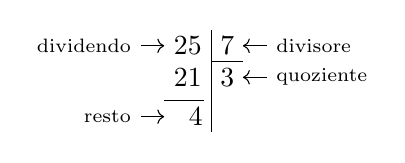
\begin{tikzpicture}

\draw[-](0,.4)--(0,-.9); % verticale
\draw[-](0,0)--(.4,0) ; %orizzontale
\draw (-.1,-.5) -- (-.6,-.5); % resto

\node (a) at (.2,.2) {7};
\node (b) at (.2,-.2) {3};
\node (c) at (-.3,.2) {25};
\node (d) at (-.3,-.2) {21};
\node (e) at (-.2,-.7){4};

\begin{scope}[font=\scriptsize]
  \draw  [<-] (.4,.2)--(.7,.2) node[right] {divisore};
  \draw  [<-] (.4,-.2)--(.7,-.2) node[right] {quoziente};
  \draw  [<-] (-.6,.2)--(-.9,.2) node[left] {dividendo};
  \draw  [<-] (-.6,-.7)--(-.9,-.7) node[left] {resto};
\end{scope}

\end{tikzpicture}

\end{center}

\end{center}
 \item 
 Ripetiamo il procedimento tra il resto parziale ottenuto, 
 $-4x^{3}+x^{2}+5x-1$ e il divisore~$3x^{2}+0x-1$. Dividiamo il primo termine 
 del resto che
 è~$-4x^{3}$ per il primo termine del divisore che è~$3x^{2}$. 
 Otteniamo~$-{\frac{4}{3}}x$ che è il secondo termine del quoziente.

\begin{center}
 % (c) 2012 Dimitrios Vrettos - d.vrettos@gmail.com

\begin{tikzpicture}[font=\small]

\matrix  (a) [matrix of  nodes, anchor=south, minimum width=9mm, nodes={text depth=2.5mm}]{
$3x^4$&$-4x^3$&$+0x^2$&$+5x$&$-1$ &$3x^2$&$+0x$&$-1$\\
$-3x^4$&$-0x^3$&$+x^2$&&{}&$x^2$&$-\displaystyle\frac{4}{3}x$\\
{}&$-4x^3$&$+x^2$&$+5x$&$-1$\\};

\draw(a-1-6.north west)--(a-2-6.south west);
  \draw(a-1-6.south west)--(a-1-8.south east);
 \draw (a-2-1.south west) -- (a-2-5.south east);

\end{tikzpicture}

\end{center}
 \item 
 Proseguiamo moltiplicando~$-{\frac{4}{3}}x$ per~$B(x)$, riportiamo il 
 risultato del prodotto, con segno opposto, sotto i
 termini del primo resto parziale e addizioniamo i due polinomi.
\begin{center}
 % (c) 2012 Dimitrios Vrettos - d.vrettos@gmail.com
\begin{tikzpicture}[font=\small]

\matrix  (a) [matrix of  nodes, anchor=south, minimum width=9mm, ,nodes={text depth=2.5mm}]{
$3x^4$&$-4x^3$&$+0x^2$&$+5x$&$-1$ &$3x^2$&$+0x$&$-1$\\
$-3x^4$&$-0x^3$&$+x^2$&&{}&$x^2$&$-\displaystyle\frac{4}{3}x$\\
{}&$-4x^3$&$+x^2$&$+5x$&$-1$\\
{}&$-4x^3$&$+0x^2$&$-\displaystyle\frac{4}{3}x$&{}\\
{}&&$x^2$&$+\displaystyle\frac{11}{3}x$&$-1$\\};

 \draw(a-1-6.north west)--(a-2-6.south west);
 \draw(a-1-6.south west)--(a-1-8.south east);
 \draw (a-2-1.south west) -- (a-2-5.south east);
\draw (a-4-2.south west) -- (a-4-5.south east);
\end{tikzpicture}
\end{center}
 \item 
 Possiamo ripetere per l'ultima volta il procedimento precedente tra il 
 resto parziale~$R_{p}(x)=x^{2}+\frac{11}{3}x-1$ e
 il divisore~$B(x)$ in quanto hanno lo stesso grado. Dividendo il termine di 
 grado maggiore di~$R_{p}(x)$, che è~$x^{2}$,
 per il termine di grado maggiore di~$B(x)$ che è~$3x^{2}$ si 
 ottiene~$\frac{1}{3}$ che è il terzo termine del polinomio quoziente.
\begin{center}
 % (c) 2012 Dimitrios Vrettos - d.vrettos@gmail.com
\begin{tikzpicture}[font=\small]

\matrix  (a) [matrix of  nodes, anchor=south, minimum width=9mm, ,nodes={text depth=2.5mm}]{
$3x^4$&$-4x^3$&$+0x^2$&$+5x$&$-1$ &$3x^2$&$+0x$&$-1$\\
$-3x^4$&$-0x^3$&$+x^2$&&{}&$x^2$&$-\displaystyle\frac{4}{3}x$&$+\displaystyle\frac{1}{3}$\\
{}&$-4x^3$&$+x^2$&$+5x$&$-1$\\
{}&$+4x^3$&$+0x^2$&$-\displaystyle\frac{4}{3}x$&{}\\
{}&&$x^2$&$+\displaystyle\frac{11}{3}x$&$-1$\\
{}&&$-x^2$&$+0x$&$+\displaystyle\frac{1}{3}$\\
{}&&&$+\displaystyle\frac{11}{3}x$&$-\displaystyle\frac{2}{3}$\\};

 \draw(a-1-6.north west)--(a-2-6.south west);
 \draw(a-1-6.south west)--(a-1-8.south east);
 \draw (a-2-1.south west) -- (a-2-5.south east);
\draw (a-4-2.south west) -- (a-4-5.south east);
\draw (a-6-4.south west) -- (a-6-5.south east);
\end{tikzpicture}
\end{center}
\end{enumerate*}

% \paragraph{Passo I}
%  Disponiamo i polinomi secondo il seguente schema, del tutto simile a quello 
%  usato per la divisione tra numeri.
% \begin{center}
%  % (c) 2012 Dimitrios Vrettos - d.vrettos@gmail.com
\begin{tikzpicture}[font=\small]

\matrix  (a) [matrix of  nodes, anchor=south,text depth=1mm]{
$3x^4$&$-4x^3$&$+0x^2$&$+5x$&$-1$ &$3x^2$&$+0x$&$-1$\\};

\draw(a-1-6.north west)--(a-1-6.south west);
\draw(a-1-6.south west)--(a-1-8.south east);

\begin{scope}[font=\scriptsize]
 \node[above] (d) at (a-1-3.north) {dividendo};
 \node[below] (r) at (a-1-3.south) {Spazio per i calcoli};
 \node [above](di) at (a-1-7.north) {divisore};
 \node [below] (q) at (a-1-7.south) {Spazio per il quoziente};
\end{scope}
\end{tikzpicture}
% \end{center}
% \paragraph{Passo II}
%  Dividiamo il primo termine del dividendo per il primo termine del divisore, 
%  otteniamo~$x^{2}$ che è il primo termine del quoziente;
%  esso va riportato nello spazio dedicato al quoziente.
% \begin{center}
%  % (c) 2012 Dimitrios Vrettos - d.vrettos@gmail.com
\begin{tikzpicture}[font=\small]
 \pgfsetmatrixrowsep{5mm}

\matrix  (a) [matrix of  nodes, anchor=south, minimum width=9mm, ,nodes={text depth=1mm}]{
$3x^4$&$-4x^3$&$+0x^2$&$+5x$&$-1$ &$3x^2$&$+0x$&$-1$\\
&&&&&$x^2$\\};

 \draw(a-1-6.north west)--(a-2-6.south west);
 \draw(a-1-6.south west)--(a-1-8.south east);

 \begin{scope}[->,red]
\draw (a-1-1.north) .. controls +(up:1cm) and +(up:1.5cm).. node[above] {$:$} (a-1-6);
\draw (a-1-6.south) -- (a-2-6.north);
 \end{scope}

\end{tikzpicture}
% \end{center}
% \paragraph{Passo III}
%  Moltiplichiamo il primo termine ottenuto per tutti i termini del divisore e 
%  trascriviamo il risultato del prodotto sotto il dividendo,
%  avendo cura, per essere facilitati nel calcolo, di:
% \begin{itemize*}
% \item incolonnare i termini con lo stesso grado, ossia scrivere i risultati 
% del prodotto in ordine da sinistra verso destra;
% \item cambiare tutti i segni ottenuti, in questo modo risulta più pratico 
% eseguire la somma algebrica dei polinomi invece della sottrazione.
% \end{itemize*}
% \begin{center}
%  % (c) 2012 Dimitrios Vrettos - d.vrettos@gmail.com
\begin{tikzpicture}[font=\small]
\pgfsetmatrixrowsep{2mm}

\matrix  (a) [matrix of  nodes, anchor=south, minimum width=9mm, text depth=1mm]{
$3x^4$&$-4x^3$&$+0x^2$&$+5x$&$-1$ &$3x^2$&$+0x$&$-1$\\
$-3x^4$&$-0x^3$&$+x^2$&&&$x^2$\\};

 \draw(a-1-6.north west)--(a-2-6.south west);
\draw(a-1-6.south west)--(a-1-8.south east);

\begin{scope}[->,red, dashed]
 \draw (a-1-7.south) -- (a-2-6.east);
  \draw (a-2-6.west) -- (a-2-3.east);
 \end{scope}

\end{tikzpicture}

% \end{center}
% \paragraph{Passo IV}
%  Sommiamo il dividendo con il polinomio sottostante e riportiamo il risultato 
%  in un'altra riga. Questo polinomio si chiama primo resto parziale.
%  Notiamo che ha grado~$3$, maggiore del grado~$2$ del divisore, pertanto la 
%  divisione va continuata.
% 
% \begin{center}
%  % (c) 2012 Dimitrios Vrettos - d.vrettos@gmail.com

\begin{center}
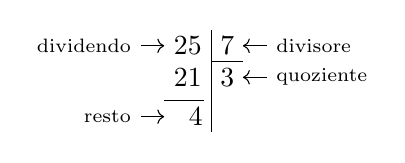
\begin{tikzpicture}

\draw[-](0,.4)--(0,-.9); % verticale
\draw[-](0,0)--(.4,0) ; %orizzontale
\draw (-.1,-.5) -- (-.6,-.5); % resto

\node (a) at (.2,.2) {7};
\node (b) at (.2,-.2) {3};
\node (c) at (-.3,.2) {25};
\node (d) at (-.3,-.2) {21};
\node (e) at (-.2,-.7){4};

\begin{scope}[font=\scriptsize]
  \draw  [<-] (.4,.2)--(.7,.2) node[right] {divisore};
  \draw  [<-] (.4,-.2)--(.7,-.2) node[right] {quoziente};
  \draw  [<-] (-.6,.2)--(-.9,.2) node[left] {dividendo};
  \draw  [<-] (-.6,-.7)--(-.9,-.7) node[left] {resto};
\end{scope}

\end{tikzpicture}

\end{center}

% \end{center}
% \paragraph{Passo V}
%  Ripetiamo il procedimento tra il resto parziale ottenuto, 
%  $-4x^{3}+x^{2}+5x-1$ e il divisore~$3x^{2}+0x-1$. Dividiamo il primo termine 
%  del resto che
%  è~$-4x^{3}$ per il primo termine del divisore che è~$3x^{2}$. 
%  Otteniamo~$-{\frac{4}{3}}x$ che è il secondo termine del quoziente.
% 
% \begin{center}
%  % (c) 2012 Dimitrios Vrettos - d.vrettos@gmail.com

\begin{tikzpicture}[font=\small]

\matrix  (a) [matrix of  nodes, anchor=south, minimum width=9mm, nodes={text depth=2.5mm}]{
$3x^4$&$-4x^3$&$+0x^2$&$+5x$&$-1$ &$3x^2$&$+0x$&$-1$\\
$-3x^4$&$-0x^3$&$+x^2$&&{}&$x^2$&$-\displaystyle\frac{4}{3}x$\\
{}&$-4x^3$&$+x^2$&$+5x$&$-1$\\};

\draw(a-1-6.north west)--(a-2-6.south west);
  \draw(a-1-6.south west)--(a-1-8.south east);
 \draw (a-2-1.south west) -- (a-2-5.south east);

\end{tikzpicture}

% \end{center}
% \paragraph{Passo VI}
%  Proseguiamo moltiplicando~$-{\frac{4}{3}}x$ per~$B(x)$, riportiamo il 
%  risultato del prodotto, con segno opposto, sotto i
%  termini del primo resto parziale e addizioniamo i due polinomi.
% \begin{center}
%  % (c) 2012 Dimitrios Vrettos - d.vrettos@gmail.com
\begin{tikzpicture}[font=\small]

\matrix  (a) [matrix of  nodes, anchor=south, minimum width=9mm, ,nodes={text depth=2.5mm}]{
$3x^4$&$-4x^3$&$+0x^2$&$+5x$&$-1$ &$3x^2$&$+0x$&$-1$\\
$-3x^4$&$-0x^3$&$+x^2$&&{}&$x^2$&$-\displaystyle\frac{4}{3}x$\\
{}&$-4x^3$&$+x^2$&$+5x$&$-1$\\
{}&$-4x^3$&$+0x^2$&$-\displaystyle\frac{4}{3}x$&{}\\
{}&&$x^2$&$+\displaystyle\frac{11}{3}x$&$-1$\\};

 \draw(a-1-6.north west)--(a-2-6.south west);
 \draw(a-1-6.south west)--(a-1-8.south east);
 \draw (a-2-1.south west) -- (a-2-5.south east);
\draw (a-4-2.south west) -- (a-4-5.south east);
\end{tikzpicture}
% \end{center}
% \paragraph{Passo VII}
%  Possiamo ripetere per l'ultima volta il procedimento precedente tra il 
%  resto parziale~$R_{p}(x)=x^{2}+\frac{11}{3}x-1$ e
%  il divisore~$B(x)$ in quanto hanno lo stesso grado. Dividendo il termine di 
%  grado maggiore di~$R_{p}(x)$, che è~$x^{2}$,
%  per il termine di grado maggiore di~$B(x)$ che è~$3x^{2}$ si 
%  ottiene~$\frac{1}{3}$ che è il terzo termine del polinomio quoziente.
% \begin{center}
%  % (c) 2012 Dimitrios Vrettos - d.vrettos@gmail.com
\begin{tikzpicture}[font=\small]

\matrix  (a) [matrix of  nodes, anchor=south, minimum width=9mm, ,nodes={text depth=2.5mm}]{
$3x^4$&$-4x^3$&$+0x^2$&$+5x$&$-1$ &$3x^2$&$+0x$&$-1$\\
$-3x^4$&$-0x^3$&$+x^2$&&{}&$x^2$&$-\displaystyle\frac{4}{3}x$&$+\displaystyle\frac{1}{3}$\\
{}&$-4x^3$&$+x^2$&$+5x$&$-1$\\
{}&$+4x^3$&$+0x^2$&$-\displaystyle\frac{4}{3}x$&{}\\
{}&&$x^2$&$+\displaystyle\frac{11}{3}x$&$-1$\\
{}&&$-x^2$&$+0x$&$+\displaystyle\frac{1}{3}$\\
{}&&&$+\displaystyle\frac{11}{3}x$&$-\displaystyle\frac{2}{3}$\\};

 \draw(a-1-6.north west)--(a-2-6.south west);
 \draw(a-1-6.south west)--(a-1-8.south east);
 \draw (a-2-1.south west) -- (a-2-5.south east);
\draw (a-4-2.south west) -- (a-4-5.south east);
\draw (a-6-4.south west) -- (a-6-5.south east);
\end{tikzpicture}
% \end{center}

Non possiamo più ripetere l'algoritmo poiché il resto ottenuto ha grado minore 
del grado del divisore.

In conclusione~$A(x):B(x)$ ha 
quoziente~$Q(x)=x^{2}-\dfrac{4}{3}x+\dfrac{1}{3}$ e 
resto~$R(x)=+{\dfrac{11}{3}}x-\dfrac{2}{3}$.

\paragraph{Verifica}
Verifichiamo se abbiamo svolto correttamente i calcoli; dovrebbe risultare, 
come detto sopra:$\quad A(x)=Q(x)\cdot B(x)+R(x)$.
\begin{equation*}
\begin{split}
\left(3x^{2}-1\right)\left(x^{2}-\frac{4}{3}x+\frac{1}{3}\right)+
\frac{11}{3}x-\frac{2}{3} & 
   = 3x^{4}-4x^{3}+x^{2}-x^{2}+\frac{4}{3}x-\frac{1}{3}+
     \frac{11}{3}x-\frac{2}{3}\\
  &= 3x^{4}-4x^{3}+\frac{15}{3}x-\frac{3}{3}\\
  &= 3x^{4}-4x^{3}+5x-1 = A(x).
\end{split}
\end{equation*}
I polinomi~$Q(x)$ e~$R(x)$ soddisfano quindi le nostre richieste. 
Ma sono unici? È sempre possibile trovarli? 
A queste domande risponde il seguente teorema.
 \end{esempio}
% \end{exrig}

\begin{teorema}[Divisione euclidea]
 Siano~$A(x)$ e~$B(x)$ due polinomi in una sola variabile, esistono e sono 
 unici due polinomi~$Q(x)$ e~$R(x)$, con grado di~$R(x)$
 minore o uguale del grado di~$B(x)$, tali che~$A(x)=Q(x)\cdot B(x)+R(x)$.
\end{teorema}

\osservazione Nel caso in cui il grado di~$A(x)$ sia minore del grado 
di~$B(x)$ il teorema resta valido, in questo caso~$Q(x)=0$ e~$R(x)=A(x)$.
Nel caso di polinomi in più variabili il teorema della divisione euclidea non 
vale.

\begin{definizione}
 Si dice che un polinomio~$A$ (dividendo) è divisibile per un polinomio~$B$ 
 (divisore) se esiste un polinomio~$Q$ (quoziente) per il quale~$A=Q\cdot B$.
\end{definizione}

% \begin{exrig}
 \begin{esempio}
 Eseguiamo la divisione tra~$A(x)=x^{3}-2x^{2}+x-2$ e~$B(x)=x^{2}+1$.
I due polinomi sono ordinati secondo potenze decrescenti della variabile, 
il grado di~$A$ è maggiore del grado di~$B$ e quest'ultimo
deve essere completo. Inseriamoli nello schema per eseguire l'algoritmo. 
Risulta:
$\left(x^{3}-2x^{2}+x-2\right):\left(x^{2}+1\right)=(x-2)$ 
il resto~$R(x)$ è il polinomio nullo e~$A(x)$ è divisibile per~$B(x)$.
Infatti~$\left(x^{2}+1\right)\cdot (x-2)=\left(x^{3}-2x^{2}+x-2\right)$.
\begin{center}
 % (c) 2012 Dimitrios Vrettos - d.vrettos@gmail.com
\begin{tikzpicture}[font=\small]

\matrix  (a) [matrix of  nodes, anchor=south, minimum width=9mm,nodes={text depth=1mm}]{
$x^3$&$-2x^2$&$+x$&$-2$ &$x^2$&$+0x$&$+1$\\
$-x^3$&$-0x^2$&$-x$&{}&$x$&$-2$\\
{}&$-2x^2$&$+0x$&$-2$\\
{}&$-2x^2$&$+0x$&$-2$\\
&&&$0$&{}\\
};

\draw(a-1-5.north west)--(a-2-5.south west);
\draw(a-1-5.south west)--(a-1-7.south east);
 \draw (a-2-1.south west) -- (a-2-4.south east);
 \draw (a-4-2.south west) -- (a-4-4.south east);
\end{tikzpicture}\vspace*{-1.10ex}
\end{center}
 \end{esempio}
% \end{exrig}

In conclusione, se~$A(x)$ è un polinomio di grado~$n$ e~$B(x)$ un polinomio 
di grado~$m$ con~$n\ge m$, quando si esegue la divisione tra~$A$ e~$B$ si 
ottiene un polinomio quoziente~$Q(x)$ di grado~$n-m$ e un polinomio~$R(x)$ 
di grado~$g<m$.
Si dimostra che i polinomi~$Q(x)$ e~$R(x)$ sono unici.

Se~$R(x)$ è il polinomio nullo, la divisione è esatta e il polinomio~$A$ è 
divisibile per il polinomio~$B$.
Se~$n<m$, allora la divisione non si può eseguire e si ottiene la frazione 
algebrica~$\frac{A}{B}$.

% \vspazio\ovalbox{\risolvii \ref{ese:12.1}, \ref{ese:12.2}, \ref{ese:12.3}, 
% \ref{ese:12.4}, \ref{ese:12.5}}

% \section{Polinomi in più variabili}
% Per la divisione tra polinomi in più variabili riportiamo soltanto qualche 
% esempio
% % \begin{exrig}
%  \begin{esempio}
% Siano~$A(a,b)=3a^{2}b+4ab^{2}+3a^{3}-2b^{3}$ e~$B(a,b)=a-3b$ rispettivamente 
% dividendo e divisore di una divisione tra polinomi;
% essi sono due polinomi omogenei nelle due variabili~$a$ e~$b$ rispettivamente 
% di grado~$3$ e grado~$1$.
% 
% Per eseguire la divisione procediamo come nel caso di polinomi in una sola 
% variabile.
% Dividiamo il polinomio~$A(a,b)=3a^{2}b+4ab^{2}+3a^{3}-2b^{3}$ per il 
% polinomio~$B(a,b)=a-3b$ rispetto alla variabile~$a$.
% Controlliamo le condizioni:
% \begin{itemize*}
% \item $A$ e~$B$ sono ordinati rispetto alla variabile a? No. $A$ non lo è. 
% Quindi ordiniamo~$A$:
% \[A(a,b)=3a^{3}+3a^{2}b+4ab^{2}-2b^{3};\]
% \item il grado di~$A$ è maggiore o uguale al grado di~$B$? Sì;
% \item $A$ e~$B$ sono completi rispetto alla variabile~$a$? Sì.
% \end{itemize*}
% Costruiamo lo schema per eseguire l'algoritmo e procediamo:
% \begin{center}
%  % (c) 2012 Dimitrios Vrettos - d.vrettos@gmail.com
\begin{tikzpicture}[x=10mm, y=10mm]

\node[circle, minimum height=2cm,draw] (A) at (0,0) {};

\node[above] (A1) at (A.north) {$A$};

\begin{scope}[fill=CornflowerBlue]

\filldraw (.5,.5) circle (2pt) node (a) {};
\node[left] at (.5,.5) {1};
\filldraw (.8,.2) circle (2pt) node (b) {};
\node[left] at (.8,.2) {2};
\filldraw (-.4,-.5) circle (2pt) node (c) {};
\node[left] at (-.4,-.5)  {3};
\filldraw (-.5,0) circle (2pt);
\node[left] at (-.5,0)  {4};
\filldraw (-.3,.5) circle (2pt);
\node[left] at (-.3,.5)  {5};
\end{scope}

\begin{scope}[xshift=2.3cm]
\node[circle, minimum height=2cm,draw] (B) at (0,0) {};

\node[above] (B1) at (B.north) {$B$};

\begin{scope}[fill=LimeGreen]
\filldraw (-.1,.6) circle (2pt) node (a1) {};
\filldraw (-.2,.2) circle (2pt)node (b1) {};
\filldraw (.2,-.7) circle (2pt) node (c1) {};
\filldraw(.5,-.2) circle (2pt);

\node[right]  at (-.1,.6) {$a$};
\node[right] at (-.2,.2) {$b$};
\node[right]  at (.2,-.7) {$c$};
\node[right] at (.5,-.2) {$d$};
\end{scope}
\end{scope}

\begin{scope}[->,smooth,thick]
\draw[Maroon] (a) .. controls +(30:1cm) and +(150:.5cm) .. (a1);
\draw[purple] (b) .. controls +(30:.5cm) and +(180:0.5cm) .. (b1);
\draw[orange] (c) .. controls +(30:1cm) and +(-90:1cm) .. (b1);
\draw[orange] (c) .. controls +(30:1cm) and +(-180:2cm) .. (c1);
\end{scope}

\begin{scope}[yshift=-2.5cm]
\matrix (m) [matrix of nodes]
{$\Dom=$&\ldots\\
$\Cod=$&\ldots\\
$\ID=$&\ldots\\
$\IM=$&\ldots\\
Tipo$=$&\ldots\\};
\end{scope}


\begin{scope}[xshift=4.6cm]

\node[circle, minimum height=2cm,draw] (A) at (0,0) {};

\node[above] (A1) at (A.north) {$A$};

\begin{scope}[fill=CornflowerBlue]

\filldraw (0,.7) circle (2pt) node (a) {};
\node[left] at (0,.7) {$a$};
\filldraw (.7,0) circle (2pt) node (b) {};
\node[left] at (.7,0) {$b$};
\filldraw (-.4,-.5) circle (2pt) node (c) {};
\node[left] at (-.4,-.5)  {$c$};
\end{scope}

\begin{scope}[xshift=2.3cm]
\node[circle, minimum height=2cm,draw] (B) at (0,0) {};

\node[above] (B1) at (B.north) {$B$};

\begin{scope}[fill=LimeGreen]
\filldraw (-.1,.6) circle (2pt) node (a1) {};
\filldraw (-.2,.2) circle (2pt)node (b1) {};
\filldraw (.2,-.7) circle (2pt) node (c1) {};

\node[right]  at (-.1,.6) {$m$};
\node[right] at (-.2,.2) {$n$};
\node[right]  at (.2,-.7) {$p$};
\end{scope}
\end{scope}

\begin{scope}[->,smooth,thick]
\draw[Maroon] (a) .. controls +(30:1cm) and +(180:1cm) .. (b1);
\draw[purple] (b) .. controls +(30:1cm) and +(180:1cm) .. (c1);
\draw[orange] (c) .. controls +(30:.5cm) and +(-180:2cm) .. (a1);
\end{scope}

\begin{scope}[yshift=-2.5cm]
\matrix (m) [matrix of nodes]
{$\Dom=$&\ldots\\
$\Cod=$&\ldots\\
$\ID=$&\ldots\\
$\IM=$&\ldots\\
Tipo$=$&\ldots\\};
\end{scope}
\end{scope}

\begin{scope}[xshift=9.2cm]
\node[circle, minimum height=2.cm,draw] (A) at (0,0) {};

\node[above] (A1) at (A.north) {$A$};

\begin{scope}[fill=CornflowerBlue]

\filldraw (.3,.7) circle (2pt) node (a) {};
\node[left] at (.3,.7) {1};
\filldraw (.6,.2) circle (2pt) node (b) {};
\node[left] at (.6,.2) {2};
\filldraw (-.3,-.5) circle (2pt) node (c) {};
\node[left] at (-.3,-.5)  {3};
\filldraw (-.5,0) circle (2pt) node (d){};
\node[left] at (-.5,0)  {4};

\end{scope}

\begin{scope}[xshift=2.3cm]
\node[circle, minimum height=2cm,draw] (B) at (0,0) {};

\node[above] (B1) at (B.north) {$B$};

\begin{scope}[fill=LimeGreen]
\filldraw (-.1,.6) circle (2pt) node (a1) {};
\filldraw (-.2,.2) circle (2pt)node (b1) {};
\filldraw (.1,-.8) circle (2pt) node (c1) {};
\filldraw(.5,-.1) circle (2pt) node (d1) {};
\filldraw(-.7,-.4) circle (2pt) node (e1) {};

\node[right]  at (-.1,.6) {$a$};
\node[right] at (-.2,.2) {$b$};
\node[right]  at (.1,-.8) {$c$};
\node[right] at (.5,-.1) {$d$};
\node[right] at (-.7,-.4) {$e$};
\end{scope}
\end{scope}

\begin{scope}[->,smooth,thick]
\draw[Maroon] (a) .. controls +(30:.5cm) and +(90:.5cm) .. (e1);
\draw[purple] (b) .. controls +(30:.5cm) and +(90:.5cm) .. (e1);
\draw[orange] (c) .. controls +(30:.5cm) and +(-180:2cm) .. (b1);
\draw[red] (d) .. controls +(-30:2cm) and +(-120:1cm) .. (d1);
\end{scope}

\begin{scope}[yshift=-2.5cm]
\matrix (m) [matrix of nodes]
{$\Dom=$&\ldots\\
$\Cod=$&\ldots\\
$\ID=$&\ldots\\
$\IM=$&\ldots\\
Tipo$=$&\ldots\\};
\end{scope}
\end{scope}
\end{tikzpicture}
% \end{center}
% Il quoziente è~$Q =\ldots \ldots \ldots$ il resto~$R = 118b^{3}$
% 
% Verifica~$\ldots \ldots \ldots \ldots \ldots \ldots$
% 
% Se avessimo eseguito la divisione rispetto alla variabile~$b$, avremmo 
% ottenuto stesso quoziente e stesso resto? Proviamo.
% Controlliamo le condizioni:
% \begin{itemize*}
% \item $A$ e~$B$ sono ordinati rispetto alla variabile~$b$? No. Ordinando~$A$, 
% risulta:
% \[A(a,b)=-2b^{3}+4ab^{2}+3a^{2}b+3a^{3}+3a^{2}b;\]
% e ordinando~$B$, risulta
% \[B(a,b)=-3b+a;\]
% \item il grado di~$A$ è maggiore o uguale al grado di~$B$? Sì;
% \item $A$ e~$B$ sono completi rispetto alla variabile~$b$? Sì.
% \end{itemize*}
% Costruisci lo schema dell'algoritmo e concludi.
%  \end{esempio}
% % \end{exrig}
% \ovalbox{\risolvii \ref{ese:12.6}, \ref{ese:12.7}}

\subsection{Regola di Ruffini}
\label{subsec:divpol_divisione_ruffini}

Per eseguire la divisione tra due polinomi, \emph{nel caso in cui il
divisore sia di grado~1} si può applicare la regola di Ruffini.
Questa regola deriva dall'algoritmo di Euclide ma lo rende più semplice.

% \begin{procedura}
%  Dividere un polinomio con la regola di Ruffini:
% 
%  \begin{enumeratea}
%  \item calcolo del resto;
% \item applicazione del procedimento di divisione;
% \item verifica.
%  \end{enumeratea}
% \end{procedura}

Partiamo da un esempio e eseguiamo innanzitutto la divisione con l'algoritmo 
di Euclide:

% ( 3 x^4 +8 x^3 +9 x^2 +4 x -5 ) : ( x +2 ) = 3 x^3 +2 x^2 +5 x -6, R= 7 %

\[\left(3 x^4 +8 x^3 +9 x^2 +4 x -5\right) : (x + 2)\]

Utilizzando l'algoritmo di Euclide otteniamo:

\begin{inaccessibleblock}[Algoritmo euclideo della divisione per i polinomi]
% \vspace{-2ex}
\begin{center}
 % (c) 2012 Dimitrios Vrettos - d.vrettos@gmail.com
\begin{tikzpicture}[font=\small]

\matrix  (a) [matrix of  nodes, anchor=south, minimum width=9mm,nodes={text depth=0mm}]{
$ 3x^4$ & $+8x^3$ & $+9x^2$ & $ +4x$ & $ -5$  & $ x   $ & $+2$    &  {}   &  {}  \\
$-3x^4$ & $-6x^3$ &    {}   &   {}   &   {}   & $ 3x^3$ & $+2x^2$ & $+5x$ & $ -6$\\
  {}    & $+2x^3$ & $+9x^2$ &   {}   &       \\
  {}    & $-2x^3$ & $-4x^2$ &   {}   &   {}   &   {}    &  R$=+7$\\
  {}    &   {}    & $+5x^2$ & $ +4x$ &   {}  \\
  {}    &   {}    & $-5x^2$ & $-10x$ &   {}  \\
  {}    &   {}    & $ {}  $ & $ -6x$ & $ -5$ \\
  {}    &   {}    & $ {}  $ & $ +6x$ & $+12$ \\
  {}    &   {}    & $ {}  $ & $ {} $ & $+7$ \\
};

\draw(a-1-5.north east)--(a-9-5.south east);
\draw(a-2-6.north west)--(a-2-9.north east);
\draw (a-2-1.south west) -- (a-2-3.south east);
\draw (a-4-2.south west) -- (a-4-4.south east);
\draw (a-6-3.south west) -- (a-6-5.south east);
\draw (a-8-4.south west) -- (a-8-5.south east);
%  \draw (a-4-2.south west) -- (a-4-4.south east);
\end{tikzpicture}
\end{center}
% \vspace*{-1.10ex}
% \vspace{-2ex}
\end{inaccessibleblock}

Possiamo osservare che la parte letterale è facilmente ricostruibile, se 
abbiamo messo per bene in colonna, e molti coefficienti sono inutilmente 
ripetuti. Riscriviamo la divisione senza la parte letterale e con i
coefficienti essenziali riquadrati:

\begin{inaccessibleblock}[Solo i coefficienti della divisione tra polinomi.]
% \vspace{-2ex}
\begin{center}
 % (c) 2012 Dimitrios Vrettos - d.vrettos@gmail.com
% (c) 2015 Daniele Zambelli - daniel.zambelli@gmail.com

\begin{tikzpicture}[font=\small, %minimum size=6mm,
data/.style={
rectangle,
minimum size=6mm,
top color=white,
bottom color=red!50!black!20,
% font=\small
},
interm/.style={
rectangle,
minimum size=6mm,
draw=black,
% font=\small
},
result/.style={
rectangle, rounded corners=3mm,
minimum size=6mm,
draw=black,
% font=\small
}]
% \begin{tikzpicture}[font=\small]

\matrix  (a) [matrix of  nodes, anchor=south, minimum width=9mm,
              nodes={text depth=0mm}]{
\node[result, data]{$+3$}; & \node[data]{$+8$}; & \node[data]{$+9$}; & 
\node[data]{$ +4$}; & \node[data]{$ -5$};  & {} &$ 1   $ & \node[data]{$+2$};    &  {}   &  {}  \\
$-3$ & \node[interm]{$-6$}; &  {}  &  {}   & {} &  {}   & $ 3$ & $+2$ & $+5$ & $ -6$\\
 {}    & \node[result]{$+2$}; & $+9$ &   {}   & {} & \\
 {}    & $-2$ & \node[interm]{$-4$}; &   {}   & {} &  {}   &   {}    &  R$=+7$\\
 {}    &  {}  & \node[result]{$+5$}; & $ +4$ &   {} & {} &\\
 {}    &  {}  & $-5$ & \node[interm]{$-10$}; &   {} & {} &\\
 {}    &  {}  & ${}$ & \node[result]{$ -6$}; & $ -5$ & {} &\\
 {}    &  {}  & ${}$ & $ +6$ & \node[interm]{$+12$}; & {} &\\
 {}    &  {}  & ${}$ & $ {}$ & \node[result]{$+7$}; & {} &\\
};

\draw(a-1-6.north east)--(a-9-6.south east);
\draw(a-2-7.north west)--(a-2-10.north east);
\draw (a-2-1.south west) -- (a-2-3.south east);
\draw (a-4-2.south west) -- (a-4-4.south east);
\draw (a-6-3.south west) -- (a-6-5.south east);
\draw (a-8-4.south west) -- (a-8-6.south east);
%  \draw (a-4-2.south west) -- (a-4-4.south east);
\end{tikzpicture}
\end{center}
% \vspace*{-1.10ex}
% \vspace{-2ex}
\end{inaccessibleblock}

In questa versione senza le variabili sono stati evidenziati i dati,
riquadrati i risultati intermedi e cerchiati i risultati.
Tutti gli altri valori sono inutili o ripetuti. La regola di Ruffini permette 
di scrivere solo i dati necessari:

\begin{inaccessibleblock}[Divisione con il metodo di Ruffini.]
% \vspace{-2ex}
\begin{center}
 % (c) 2012 Dimitrios Vrettos - d.vrettos@gmail.com
% (c) 2015 Daniele Zambelli - daniel.zambelli@gmail.com

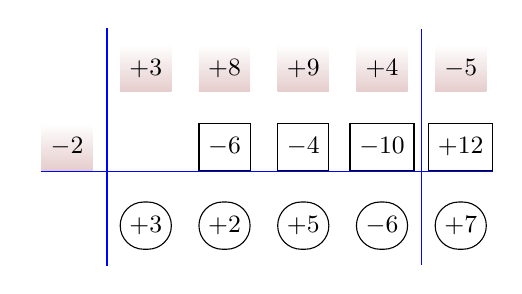
\begin{tikzpicture}[font=\small, %minimum size=6mm,
data/.style={
rectangle,
minimum size=6mm,
top color=white,
bottom color=red!50!black!20,
% font=\small
},
interm/.style={
rectangle,
minimum size=6mm,
draw=black,
% font=\small
},
result/.style={
rectangle, rounded corners=3mm,
minimum size=6mm,
draw=black,
% font=\small
},
x=10mm, y=10mm, minimum size=10mm]


% \begin{tikzpicture}[font=\small,x=8mm, y=8mm, minimum size=10mm]

\node (a0) at (0,0) {};
\node [data](a1) at (1,0) {$+3$};
\node [data](a2) at (2,0) {$+8$};
\node [data](a3) at (3,0) {$+9$};
\node [data](a4) at (4,0) {$+4$};
\node [data](a5) at (5,0) {$-5$};

\node [data](a6) at (0,-1) {$-2$};
\node (a7) at (1,-1) {};
\node [interm](a8) at (2,-1) {$-6$};
\node [interm](a9) at (3,-1) {$-4$};
\node [interm](a10) at (4,-1) {$-10$};
\node [interm](a11) at (5,-1) {+12};

\node (a12) at (0,-2) {};
\node [result](a13) at (1,-2) {$+3$};
\node [result](a14) at (2,-2) {$+2$};
\node [result](a15) at (3,-2) {$+5$};
\node [result](a16) at (4,-2) {$-6$};
\node [result](a17) at (5,-2) {$+7$};

\begin{scope}[blue]
\draw (a0.north east)--(a12.south east);
 \draw (a6.south west)--(a11.south east);
% \draw (a4.north east)--(a16.south east);
\draw (4.5, 0.5)--(4.5, -2.5);
\end{scope}

% \matrix (a)[matrix of nodes, nodes in empty cells,
%             nodes={ text width=8mm, text depth=1mm, text centered}]
% {
%  {}  & \node [data]{$+3$}; & \node [data]{$+8$}; & \node [data]{$+9$}; & \node [data]{$+4$};  & \node [data]{$-5$}; \\
% $-2$ &  {}  & $-6$ & $-4$ & $-10$ & $+12$ \\
%  {}  & $+3$ & $+2$ & $+5$ & $-6$  & $+7$  \\
% };  
% \begin{scope}[blue]
% \draw(a-1-2.north west)--(a-3-2.south west);
% \draw(a-2-1.south west)--(a-2-6.south east);
% \draw(a-1-5.north east)--(a-3-5.south east);
% \end{scope}

\end{tikzpicture}
\end{center}
% \vspace*{-1.10ex}
% \vspace{-2ex}
\end{inaccessibleblock}

Ma come si possono ottenere tutti i coefficienti senza l'algoritmo di Euclide?
Vediamo in questo caso concreto:
\begin{itemize*}
 \item $-2$ è l'opposto del termine noto del divisore;
 \item addiziono $+3$ con $0$ e ottengo $+3$;
 \item moltiplico $-2$ con $+3$ e ottengo $-6$;
 \item addiziono $+8$ con $-6$ e ottengo $+2$;
 \item moltiplico $-2$ con $+2$ e ottengo $-4$; 
 \item addiziono $+9$ con $-4$ e ottengo $+5$;
 \item moltiplico $-2$ con $+5$ e ottengo $-10$; 
 \item addiziono $+4$ con $-10$ e ottengo $-6$;
 \item moltiplico $-2$ con $-6$ e ottengo $+12$; 
 \item addiziono $-5$ con $+12$ e ottengo $+7$.
\end{itemize*}

% \begin{itemize*}
%  \item $-2$ è l'opposto del termine noto del divisore:
%  \item $+3$ è il primo coefficiente del dividendo
%  \item $-6 = -2 \cdot 3$ 
%  \item $+2 = +8 -6$ 
%  \item $-4 = -2 \cdot 2$ 
%  \item $+5 = +9 -4$ 
%  \item $-10 = -2 \cdot 5$ 
%  \item $-6 = +4 -10$ 
%  \item $+12 = -2 \cdot (-6)$ 
%  \item $+7 = (-5)+(+12)$ 
% \end{itemize*}

Come è riassunto nel seguente diagramma dove le frecce 
verdi tratteggiate indicano \emph{addizioni} e quelle 
rosse punteggiate indicano \emph{moltiplicazione}.

\begin{inaccessibleblock}[Divisione con il metodo di Ruffini.]
% \vspace{-2ex}
\begin{center}
 % (c) 2012 Dimitrios Vrettos - d.vrettos@gmail.com
% (c) 2015 Daniele Zambelli - daniel.zambelli@gmail.com

\usepgflibrary{arrows.meta}

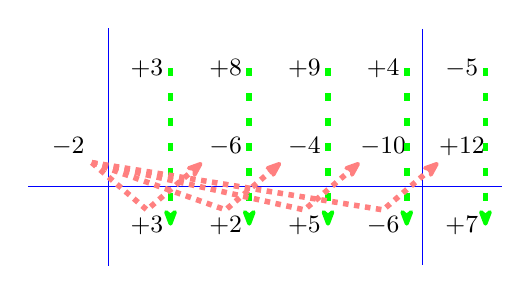
\begin{tikzpicture}[font=\small, x=10mm, y=10mm, minimum size=10mm]

% \begin{tikzpicture}[font=\small,x=8mm, y=8mm, minimum size=10mm]

\node (a0) at (0,0) {};
\node (a1) at (1,0) {$+3$};
\node (a2) at (2,0) {$+8$};
\node (a3) at (3,0) {$+9$};
\node (a4) at (4,0) {$+4$};
\node (a5) at (5,0) {$-5$};

\node (a6) at (0,-1) {$-2$};
\node (a7) at (1,-1) {};
\node (a8) at (2,-1) {$-6$};
\node (a9) at (3,-1) {$-4$};
\node (a10) at (4,-1) {$-10$};
\node (a11) at (5,-1) {+12};

\node (a12) at (0,-2) {};
\node (a13) at (1,-2) {$+3$};
\node (a14) at (2,-2) {$+2$};
\node (a15) at (3,-2) {$+5$};
\node (a16) at (4,-2) {$-6$};
\node (a17) at (5,-2) {$+7$};

\begin{scope}[blue]
\draw (a0.north east)--(a12.south east);
 \draw (a6.south west)--(a11.south east);
% \draw (a4.north east)--(a16.south east);
\draw (4.5, 0.5)--(4.5, -2.5);
\end{scope}

% \draw (a0.north east)--(a12.south east);
% \draw (a6.south west)--(a11.south east);
% \draw (a4.north east)--(a16.south east);

\draw [-{Stealth[length=3mm, open, round]}, 
       green, loosely dashed, line width=2pt](1.3, 0) -- (1.3, -2);
% \draw [-{Stealth[length=3mm, open, round]}, 
%       red, solid, line width=2pt] 
%       (a6.east) [xshift=-0.5cm] -- (a13.north) [yshift=-0.5cm] -- (a8.west) [xshift=+0.5cm];
\draw [-{Stealth[length=3mm, open, round]}, 
       red!50, dotted, line width=2pt] 
       (0.3, -1.2) -- (1, -1.8) -- (1.7, -1.2);
\draw [-{Stealth[length=3mm, open, round]}, 
       green, loosely dashed, line width=2pt](2.3, 0) -- (2.3, -2);
\draw [-{Stealth[length=3mm, open, round]}, 
       red!50, dotted, line width=2pt] 
       (0.3, -1.2) -- (2, -1.8) -- (2.7, -1.2);
\draw [-{Stealth[length=3mm, open, round]}, 
       green, loosely dashed, line width=2pt](3.3, 0) -- (3.3, -2);
\draw [-{Stealth[length=3mm, open, round]}, 
       red!50, dotted, line width=2pt] 
       (0.3, -1.2) -- (3, -1.8) -- (3.7, -1.2);
\draw [-{Stealth[length=3mm, open, round]}, 
       green, loosely dashed, line width=2pt](4.3, 0) -- (4.3, -2);
\draw [-{Stealth[length=3mm, open, round]}, 
       red!50, dotted, line width=2pt] 
       (0.3, -1.2) -- (4, -1.8) -- (4.7, -1.2);
\draw [-{Stealth[length=3mm, open, round]}, 
       green, loosely dashed, line width=2pt](5.3, 0) -- (5.3, -2);

\end{tikzpicture}
\end{center}
% \vspace*{-1.10ex}
% \vspace{-2ex}
\end{inaccessibleblock}

E aggiungendo le variabili si ottiene il risultato:

\[Q = 3 x^3 +2 x^2 +5 x -6 \quad R = +7\]

Come avevamo calcolato con l'algoritmo di Euclide.

Da notare che:
\begin{itemize*}
 \item la prima riga contiene i coefficienti del dividendo;
 \item il termine noto del dividendo e posto a destra della seconda linea 
  verticale;
 \item nella seconda riga, prima della prima linea verticale si scrive il 
  termine noto del divisore cambiato di segno, così invece di ricordarsi di 
  cambiare di segno ogni volta (come nell'algoritmo di Euclide), lo si fa una 
  volta per tutte;
 \item l'algoritmo inizia con un'addizione tra il primo coefficiente del 
  dividendo e $0$ (addizione facile);
 \item nella terza riga otteniamo i coefficienti del risultato;
 \item dividendo un polinomio di grado enne per un polinomio di primo grado 
  si ottiene un polinomio di grado $n-1$, quindi, in questo caso, il primo 
  monomio sarà di grado $2$;
 \item il termine in basso a destra è il resto della divisione, per forza di 
  grado zero;
 \item se il resto della divisione è zero vuol dire che il \emph{dividendo} è 
  un multiplo del \emph{divisore}.
\end{itemize*}


% \begin{exrig}
 \begin{esempio}
Eseguire la seguente divisione:
 
$\left(-3a+a^{3}+1\right):(a-3)$

Il divisore è del tipo $(x + x_0)$ quindi posso usare la regola di Ruffini.
Prima di tutto mettiamo in ordine il dividendo completandolo:

$\left(-3a+a^{3}+0a^2-3a+1\right):(a-3)$

Poi inseriamo i dati nello schema di Ruffini ed eseguiamo addizioni e 
moltiplicazioni. Dobbiamo ricordarci di cambiare segno al termine noto del 
divisore

\begin{inaccessibleblock}[Divisione con il metodo di Ruffini.]
% \vspace{-2ex}
\begin{center}
 % (c) 2012 Dimitrios Vrettos - d.vrettos@gmail.com
% (c) 2015 Daniele Zambelli - daniel.zambelli@gmail.com

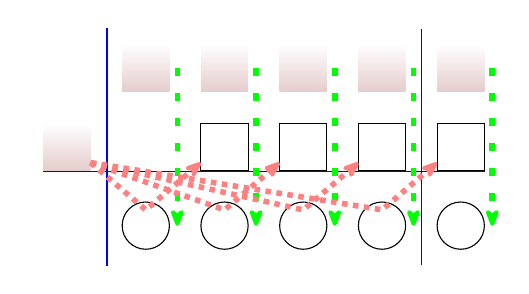
\begin{tikzpicture}[font=\small, %minimum size=6mm,
data/.style={
rectangle,
minimum size=6mm,
top color=white,
bottom color=red!50!black!20,
% font=\small
},
interm/.style={
rectangle,
minimum size=6mm,
draw=black,
% font=\small
},
result/.style={
rectangle, rounded corners=3mm,
minimum size=6mm,
draw=black,
% font=\small
},
x=10mm, y=10mm, minimum size=10mm]


% \begin{tikzpicture}[font=\small,x=8mm, y=8mm, minimum size=10mm]

\node (a0) at (0,0) {};
\node [data](a1) at (1,0) {};
\node [data](a2) at (2,0) {};
\node [data](a3) at (3,0) {};
\node [data](a4) at (4,0) {};
\node [data](a5) at (5,0) {};

\node [data](a6) at (0,-1) {};
\node (a7) at (1,-1) {};
\node [interm](a8) at (2,-1) {};
\node [interm](a9) at (3,-1) {};
\node [interm](a10) at (4,-1) {};
\node [interm](a11) at (5,-1) {};

\node (a12) at (0,-2) {};
\node [result](a13) at (1,-2) {};
\node [result](a14) at (2,-2) {};
\node [result](a15) at (3,-2) {};
\node [result](a16) at (4,-2) {};
\node [result](a17) at (5,-2) {};

% \draw (a0.north east)--(a12.south east);
%  \draw (a6.south west)--(a11.south east);
% \draw (a4.north east)--(a16.south east);

\begin{scope}[blue]
\draw (a0.north east)--(a12.south east);
 \draw (a6.south west)--(a11.south east);
% \draw (a4.north east)--(a16.south east);
\draw (4.5, 0.5)--(4.5, -2.5);
\end{scope}

\draw [-{Stealth[length=3mm, open, round]}, 
       green, loosely dashed, line width=2pt](1.4, 0) -- (1.4, -2);
\draw [-{Stealth[length=3mm, open, round]}, 
       red!50, dotted, line width=2pt] 
       (0.3, -1.2) -- (1, -1.8) -- (1.7, -1.2);
\draw [-{Stealth[length=3mm, open, round]}, 
       green, loosely dashed, line width=2pt](2.4, 0) -- (2.4, -2);
\draw [-{Stealth[length=3mm, open, round]}, 
       red!50, dotted, line width=2pt] 
       (0.3, -1.2) -- (2, -1.8) -- (2.7, -1.2);
\draw [-{Stealth[length=3mm, open, round]}, 
       green, loosely dashed, line width=2pt](3.4, 0) -- (3.4, -2);
\draw [-{Stealth[length=3mm, open, round]}, 
       red!50, dotted, line width=2pt] 
       (0.3, -1.2) -- (3, -1.8) -- (3.7, -1.2);
\draw [-{Stealth[length=3mm, open, round]}, 
       green, loosely dashed, line width=2pt](4.4, 0) -- (4.4, -2);
\draw [-{Stealth[length=3mm, open, round]}, 
       red!50, dotted, line width=2pt] 
       (0.3, -1.2) -- (4, -1.8) -- (4.7, -1.2);
\draw [-{Stealth[length=3mm, open, round]}, 
       green, loosely dashed, line width=2pt](5.4, 0) -- (5.4, -2);

\end{tikzpicture}
\end{center}
% \vspace*{-1.10ex}
% \vspace{-2ex}
\end{inaccessibleblock}

Infine scriviamo il risultato: quoziente e resto:

Q=$a^2+3a+6$; \quad R=$19$
\end{esempio}
% \end{exrig}

% \paragraph{Passo I} \emph{Calcolo del polinomio resto.}
% 
% Si considera il termine numerico del polinomio divisore cambiato di
% segno (nell'esempio è~1) e si sostituisce alla
% lettera del polinomio dividendo~$A(a)$:~$(1)^{2 }-3(1) + 1 = 1 - 3 + 1 = -1$.
% 
% Il resto della divisione è~$-1$.
% 
% \paragraph{Passo II} \emph{Applicazione del procedimento di divisione.}
% 
% Disegnare il seguente schema di Ruffini: scrivere i coefficienti
% numerici del polinomio dividendo, secondo le potenze decrescenti della
% variabile. Se manca un termine occorre mettere~0.
% L'ultimo termine numerico è messo esternamente alla
% griglia. Nell'angolo a sinistra dello schema si pone il
% termine numerico del polinomio divisore cambiato di segno,
% nell'esempio è~1.
% 
% \begin{center}
% % (c) 2012 Dimitrios Vrettos - d.vrettos@gmail.com
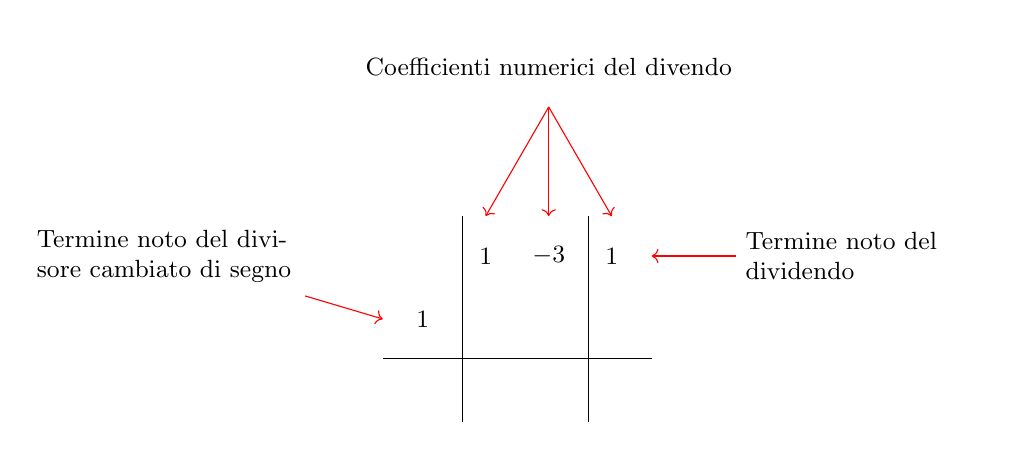
\begin{tikzpicture}[font=\small,x=8mm, y=8mm, minimum size=10mm]

\node (a0) at (0,0) {};
\node (a1) at (1,0) {1};
\node (a2) at (2,0) {$-3$};
\node (a3) at (3,0) {1};

\node(a4) at (0,-1) {1};
\node (a5) at (1,-1) {};
\node (a6) at (2,-1) {};
\node (a7) at (3,-1) {};

\node (a8) at (0,-2) {};
\node (a9) at (1,-2) {};
\node (a10) at (2,-2) {};
\node (a11) at (3,-2) {};

\draw (a0.north east)--(a8.south east);
 \draw (a4.south west)--(a7.south east);
\draw (a2.north east)--(a10.south east);

\node (b) at (2,3) {Coefficienti numerici del divendo};
\node[text width=3.4cm] (c) at (-4,0){Termine noto del divisore cambiato di segno};
\node[text width=3cm] (d) at (7,0) {Termine noto del dividendo};

\begin{scope}[->, red]
\foreach \x in {a1.north, a2.north, a3.north}
	\draw (b.south)--(\x);
\draw (c) -- (a4.west);
\draw (d)-- (a3.east);
\end{scope}

\end{tikzpicture}
% \end{center}
% 
% \begin{multicols}{2}
%  Il primo termine si riporta inalterato nella parte sottostante:
% \begin{center}
% % (c) 2012 Dimitrios Vrettos - d.vrettos@gmail.com
\begin{tikzpicture}[font=\small,x=8mm, y=8mm, minimum size=10mm]

\node (a0) at (0,0) {};
\node (a1) at (1,0) {1};
\node (a2) at (2,0) {$-3$};
\node (a3) at (3,0) {1};

\node(a4) at (0,-1) {1};
\node (a5) at (1,-1) {};
\node (a6) at (2,-1) {};
\node (a7) at (3,-1) {};

\node (a8) at (0,-2) {};
\node (a9) at (1,-2) {1};
\node (a10) at (2,-2) {};
\node (a11) at (3,-2) {};

\draw (a0.north east)--(a8.south east);
 \draw (a4.south west)--(a7.south east);
\draw (a2.north east)--(a10.south east);

\draw[->,red] (a1.south)--(a9.north);

\end{tikzpicture}
% \end{center}
% \end{multicols}
% 
% \begin{multicols}{2}
%  Moltiplicare il termine noto del divisore (cambiato di segno) per il
% primo coefficiente appena trascritto e riportare il risultato sotto il
% secondo coefficiente
% \begin{center}
% % (c) 2012 Dimitrios Vrettos - d.vrettos@gmail.com
\begin{tikzpicture}[font=\small,x=8mm, y=8mm, minimum size=10mm]

\node (a0) at (0,0) {};
\node (a1) at (1,0) {1};
\node (a2) at (2,0) {$-3$};
\node (a3) at (3,0) {1};

\node(a4) at (0,-1) {1};
\node (a5) at (1,-1) {};
\node (a6) at (2,-1) {1};
\node (a7) at (3,-1) {};

\node (a8) at (0,-2) {};
\node (a9) at (1,-2) {1};
\node (a10) at (2,-2) {};
\node (a11) at (3,-2) {};

\draw (a0.north east)--(a8.south east);
 \draw (a4.south west)--(a7.south east);
\draw (a2.north east)--(a10.south east);

\draw[->,red] (a4.south)--(a9.west);
\draw[->,red] (a9.east)--(a6.south);
\end{tikzpicture}
% \end{center}
% \end{multicols}
% 
% \begin{multicols}{2}
%  Sommare i due termini appena incolonnati~$-3+1=-2$.
% \begin{center}
% % (c) 2012 Dimitrios Vrettos - d.vrettos@gmail.com
\begin{tikzpicture}[font=\small,x=8mm, y=8mm, minimum size=10mm]

\node (a0) at (0,0) {};
\node (a1) at (1,0) {1};
\node (a2) at (2,0) {$-3$};
\node (a3) at (3,0) {1};

\node(a4) at (0,-1) {1};
\node (a5) at (1,-1) {};
\node (a6) at (2,-1) {1};
\node (a7) at (3,-1) {};

\node (a8) at (0,-2) {};
\node (a9) at (1,-2) {1};
\node (a10) at (2,-2) {$-2$};
\node (a11) at (3,-2) {};

\draw (a0.north east)--(a8.south east);
 \draw (a4.south west)--(a7.south east);
\draw (a2.north east)--(a10.south east);

\end{tikzpicture}
% \end{center}
% \end{multicols}
% 
% \begin{multicols}{2}
%  Moltiplicare il termine noto del divisore (cambiato di segno) per la
% somma appena ottenuta~$1\cdot (-2)=-2$.
% \begin{center}
% % (c) 2012 Dimitrios Vrettos - d.vrettos@gmail.com
\begin{tikzpicture}[font=\small,x=8mm, y=8mm, minimum size=10mm]

\node (a0) at (0,0) {};
\node (a1) at (1,0) {1};
\node (a2) at (2,0) {$-3$};
\node (a3) at (3,0) {1};

\node(a4) at (0,-1) {1};
\node (a5) at (1,-1) {};
\node (a6) at (2,-1) {1};
\node (a7) at (3,-1) {$-2$};

\node (a8) at (0,-2) {};
\node (a9) at (1,-2) {1};
\node (a10) at (2,-2) {$-2$};
\node (a11) at (3,-2) {};

\draw (a0.north east)--(a8.south east);
 \draw (a4.south west)--(a7.south east);
\draw (a2.north east)--(a10.south east);

\begin{scope}[->,red]
\draw (a4.east)--(a10.west);
\draw (a10.east)--(a7.south);
\end{scope}
\end{tikzpicture}

% \end{center}
% \end{multicols}
% \newpage
% \begin{multicols}{2}
%  Addizionare gli ultimi due numeri incolonnati~$1-2=-1$.
% \begin{center}
% % (c) 2012 Dimitrios Vrettos - d.vrettos@gmail.com
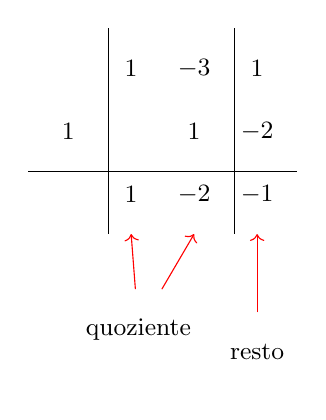
\begin{tikzpicture}[font=\small,x=8mm, y=8mm, minimum size=10mm]

\node (a0) at (0,0) {};
\node (a1) at (1,0) {1};
\node (a2) at (2,0) {$-3$};
\node (a3) at (3,0) {1};

\node(a4) at (0,-1) {1};
\node (a5) at (1,-1) {};
\node (a6) at (2,-1) {1};
\node (a7) at (3,-1) {$-2$};

\node (a8) at (0,-2) {};
\node (a9) at (1,-2) {1};
\node (a10) at (2,-2) {$-2$};
\node (a11) at (3,-2) {$-1$};

\draw (a0.north east)--(a8.south east);
 \draw (a4.south west)--(a7.south east);
\draw (a2.north east)--(a10.south east);

\node[below left of=a10,below=5mm](q)  {quoziente};
\node[below of=a11, below=5mm](r)  {resto};
\begin{scope}[->,red]
\draw (q)--(a9.south);
\draw (q)--(a10.south);
\draw (r)--(a11.south);
\end{scope}
\end{tikzpicture}
% \end{center}
% \end{multicols}
% 
% Infine si ricostruisce il polinomio quoziente, tenendo presente che i
% coefficienti numerici sono quelli trovati da questa divisione, cioè~1
% e~$-2$. Quoziente e resto sono allora~$Q(x)=a-2$ e~$R=-1$.
% 
% \paragraph{Passo III}\emph{Verifica}
% 
% Come nella divisione con i numeri si moltiplica il polinomio risultato
% per il polinomio divisore e si somma il polinomio resto. Il risultato
% deve essere il polinomio dividendo.
% \[(a - 2)(a - 1) + (-1) = a^{2} - a - 2a + 2 - 1 =a^{2}-3a + 1.\]
%  \end{esempio}
% 
% \begin{esempio}
% $(4x^{3} - 5x + 6): (x + 1).$
% 
% Applicazione del procedimento di divisione
% \begin{center}
% % (c) 2012 Dimitrios Vrettos - d.vrettos@gmail.com
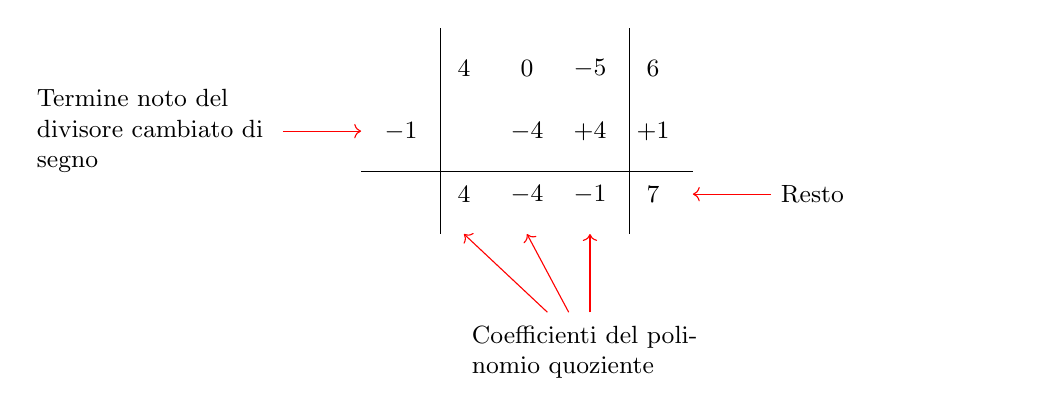
\begin{tikzpicture}[font=\small,x=8mm, y=8mm, minimum size=10mm]

\node (a0) at (0,0) {};
\node (a1) at (1,0) {4};
\node (a2) at (2,0) {0};
\node (a3) at (3,0) {$-5$};
\node (a4) at (4,0) {6};

\node(a5) at (0,-1) {$-1$};
\node (a6) at (1,-1) {};
\node (a7) at (2,-1) {$-4$};
\node (a8) at (3,-1) {$+4$};
\node (a9) at (4,-1) {$+1$};

\node (a10) at (0,-2) {};
\node (a11) at (1,-2) {4};
\node (a12) at (2,-2) {$-4$};
\node (a13) at (3,-2) {$-1$};
\node (a14) at (4,-2) {7};

\draw (a0.north east)--(a10.south east);
 \draw (a5.south west)--(a9.south east);
\draw (a3.north east)--(a13.south east);

 \node[text width=3cm, left of=a5, left=5mm](b)  {Termine noto del divisore cambiato di segno};
 \node[text width=3cm, below of=a13, below=5mm](c)  {Coefficienti del polinomio quoziente};
 \node[text width=3cm, right of=a14, right=5mm](d)  {Resto};
 \begin{scope}[->,red]
 \draw (b)--(a5.west);
 \draw (d)--(a14);
\foreach \x in {a11,a12,a13}
\draw (c)--(\x.south);
 \end{scope}
\end{tikzpicture}
% \end{center}
% \[Q(x)=4x^{2}-4x-1 \qquad R=7.\]
% \end{esempio}
% 
% \textit{Verifica.}
% 
% \[Q(x)\cdot B(x)+R=A(x)\]
% 
% \[\left(4x^{2}-4x-1\right)\cdot (x+1)+7=4x^{3}+4x^{2}-4x-x-1+7=4x^{3}-5x+6\]
% 
% Vediamo il caso in cui il binomio che fa da divisore ha coefficiente
% numerico della variabile diverso da~1.
% 
% 
% \begin{esempio}
%  Dividere con la regola di 
% Ruffini~$\left(2x^{4}-x^{3}-4x^{2}+2x+7\right):(2x-1)$.
% 
% In questo tipo di esercizi si deve rendere il divisore del tipo~$x+n$,
% quindi nel nostro caso si deve dividere sia il dividendo sia il
% divisore per~2; sappiamo, infatti, dalla proprietà invariantiva della
% divisione che dividendo per uno stesso numero dividendo e divisore il
% quoziente della divisione non cambia. Il resto invece risulterà
% diviso per~2. Quindi applichiamo l'algoritmo precedente
% e \emph{ricordiamoci al termine della divisione di moltiplicare il
% resto per}~2.
% 
% La divisione allora diventa
% 
% $\left(x^{4}-\frac{1}{2}x^{3}-2x^{2}+x+\frac{7}{2}\right):\left(x-\frac{1}{2}
% \right)$.
% \end{esempio}
% % \end{exrig}
% 
% \ovalbox{\risolvii \ref{ese:12.8}, \ref{ese:12.9}, \ref{ese:12.10}, 
% \ref{ese:12.11}, \ref{ese:12.12}}

% \subsection{Calcolo del resto}
% 
% Si considera il termine numerico del polinomio divisore cambiato di
% segno (nell'esempio è~$+{\frac{1}{2}}$) e si
% sostituisce alla lettera del polinomio dividendo. Il risultato che si
% ottiene è il resto della nuova 
% 
% divisione~$\left(\frac{1}{2}\right)^{4}-\frac{1}{2}\left(\frac{1}{2}\right)^{3}
% -2\left(\frac{1}{2}\right)^{2}+\frac{1}{2}+\frac{7}{2}=-\frac{1}{16}-\frac{1}{2}
% +\frac{1}{2}+\frac{7}{2}=\frac{7}{2}$
% resto della divisione.
% 
% Applicazione del procedimento di divisione.
% \begin{center}
%  % (c) 2012 Dimitrios Vrettos - d.vrettos@gmail.com
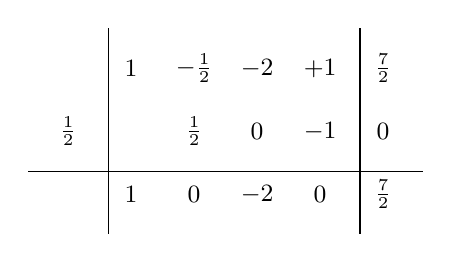
\begin{tikzpicture}[font=\small,x=8mm, y=8mm, minimum size=10mm]

\node (a0) at (0,0) {};
\node (a1) at (1,0) {1};
\node (a2) at (2,0) {$-\frac{1}{2}$};
\node (a3) at (3,0) {$-2$};
\node (a4) at (4,0) {$+1$};
\node (a5) at (5,0) {$\frac{7}{2}$};

\node(a6) at (0,-1) {$\frac{1}{2}$};
\node (a7) at (1,-1) {};
\node (a8) at (2,-1) {$\frac{1}{2}$};
\node (a9) at (3,-1) {0};
\node (a10) at (4,-1) {$-1$};
\node (a11) at (5,-1) {0};

\node (a12) at (0,-2) {};
\node (a13) at (1,-2) {1};
\node (a14) at (2,-2) {0};
\node (a15) at (3,-2) {$-2$};
\node (a16) at (4,-2) {0};
\node (a17) at (5,-2) {$\frac{7}{2}$};

\draw (a0.north east)--(a12.south east);
 \draw (a6.south west)--(a11.south east);
\draw (a4.north east)--(a16.south east);

\end{tikzpicture}
% \end{center}
% 
% Adesso si pone la lettera per ogni termine del polinomio risultato
% partendo dal grado del polinomio dividendo diminuito di~1. Il risultato
% è quindi il polinomio~$x^{3}-2x$, il resto è~$\frac{7}{2}\cdot2=7$.
% 
% \paragraph{Verifica}
% Per la proprietà della divisione si moltiplica il quoziente per il
% polinomio divisore e si somma il resto ottenuto. Il risultato deve
% essere il polinomio dividendo.
% 
% \[\left(x^{3}-2x\right)(2x-1)+7=2x^{4}-x^{3}-4x^{2}+2x+7.\]
% 
% In generale, se si vuole dividere il polinomio~$A(x)$ per il 
% binomio~$(nx-\alpha)$, utilizzando la proprietà invariantiva della
% divisione, basta dividere dividendo e divisore per~$n$. Si
% ottengono~$Q(x)$ e resto. Per ottenere il resto della divisione di
% partenza occorre moltiplicare per il coefficiente~$n$.
% Infatti si ha:~$A(x)=(nx-\alpha)Q(x)+R $
% e, dividendo ambo i membri per~$n$, si ha:
% \[\frac{A(x)}{n}=\left(x-\frac{\alpha }{n}\right)Q(x)+\frac{R}{n}.\]
% \ovalbox{\risolvii \ref{ese:12.13}, \ref{ese:12.14}, \ref{ese:12.15}, 
% \ref{ese:12.16}, \ref{ese:12.17}, \ref{ese:12.18}}

%%%%%%%%%%%%%%%%%%%%%%%%%%%%% sopstare sotto.

\subsection{Teorema di Ruffini}
\label{subsec:divpol_teorema_ruffini}

\begin{teorema}[del resto]
 Il resto della divisione di un polinomio~$A(x)$ per un
binomio del tipo~$x+k$ è uguale al valore che~$A(x)$ assume quando
al posto della variabile~$x$ si sostituisce il valore~$-k$, $R=A(-k)$.
\end{teorema}

\begin{proof}
 Dalla divisione di~$A(x)$ per~$x-k$ otteniamo la seguente
uguaglianza:
\[A(x)=(x-k)\cdot Q(x)+R\]
in cui si è scritto~$R$ anziché $R(x)$, poiché essendo il divisore di primo 
grado, il resto è di grado zero quindi è una costante.

Essendo tale relazione valida per qualsiasi valore che si attribuisce
alla variabile~$x$, sostituiamo al suo posto il valore~$-k$ e otteniamo:

\[A(-k)=(-k+k) \cdot Q(k)+R\]

Ma:

\begin{itemize*}
 \item $A(-k)=0$ per ipotesi;
 \item $(-k+k)=0$ per ovvi motivi.
\end{itemize*}

Quindi l'espressione precedente diventa:

\[0=0 \cdot Q(k)+R \quad \Longrightarrow \quad R=0 \qquad \text{q.e.d}\]

\end{proof}

Dalla:

\[A(-k)=(-k+k) \cdot Q(k)+R \Longrightarrow R=A(-k)\]

Si ottiene il seguente corollario:

Il valore assunto da~$A(x)$ quando~$x$ è sostituito da~$-k$
è uguale al \emph{resto} della divisione di~$A(x)$ per~$(x+k)$, 
cioè:~$A(-k)=R$.

Dal teorema del resto si può ottenere il

\begin{teorema}[di Ruffini]
Condizione necessaria e sufficiente affinché un polinomio~$A(x)$ 
sia divisibile per un binomio del tipo~$x+k$ è
che risulti~$A(-k)=0$.
\end{teorema}

\begin{proof}

\emph{Prima implicazione}:~$A(x)$ divisibile per~$x+k\Rightarrow A(-k)=0$.

Poiché $A(x)$ è divisibile per~$x+k$, per definizione di divisibilità deve 
essere~$R=0$. 
Ma, per il teorema del resto, $A(k)=R=0$, 
quindi, per la proprietà transitiva dell'uguaglianza, $A(-k)=0$.

\emph{Seconda implicazione}:~$A(-k)=0\Rightarrow A(x)$ divisibile per~$x+k$.

Il resto della divisione del polinomio~$A(x)$ per il binomio~$x+k$,
per il teorema del resto risulta~$R=A(-k)$ e per ipotesi~$A(k)=0$,
ne segue che~$R=0$. Per definizione di divisibilità, essendo il
resto della divisione zero, segue che~$A(x)$ è divisibile per~$x+k$.
\end{proof}

% ----------------- Scomposizione -------------------------

\section{Scomposizione in fattori}

\subsection{Cosa vuol dire scomporre in fattori}
\label{subsec:divpol_scomporre}

Scomporre un polinomio in fattori significa scrivere il polinomio come 
prodotto di polinomi e monomi che
moltiplicati tra loro diano come risultato il polinomio stesso. 
Si può paragonare la scomposizione in fattori
di un polinomio alla scomposizione in fattori dei numeri naturali.

\begin{minipage}{.4\textwidth}
\begin{inaccessibleblock}[Grafo ad albero della scomposizione del numero 42]
 \begin{center}
 % (c) 2014 Daniele Zambelli - daniele.zambelli@gmail.com

\begin{tikzpicture}[level/.style={sibling distance=30mm/#1, level distance=8mm}]
\node {$\qquad \qquad 42 = 2 \cdot 3 \cdot 7$}
  child {node {$7$}}
  child {node {$6$}
    child {node {$2$}}
    child {node {$3$}}
  };
\end{tikzpicture}

 \end{center}
\end{inaccessibleblock}
\end{minipage}
\begin{minipage}{.6\textwidth}
\begin{inaccessibleblock}[Grafo ad albero della scomposizione del 
polinomio:~$3a^{3}b^{2}-3ab^{4}$]
 \begin{center}
 % (c) 2014 Daniele Zambelli - daniele.zambelli@gmail.com

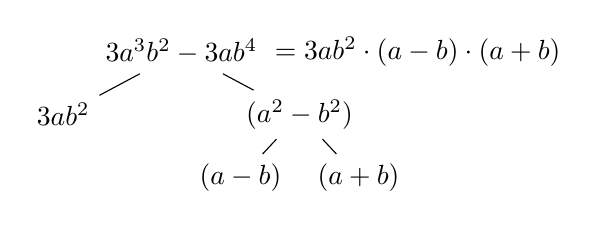
\begin{tikzpicture}[level/.style={sibling distance=30mm/#1, level distance=8mm}]
% \node {$ \qquad \qquad \qquad \qquad \qquad 
%         3a^{3}b^{2}-3ab^{4} = 3ab^2 \cdot (a-b) \cdot (a+b)$}
\node {$3a^{3}b^{2}-3ab^{4}$}
  child {node {$3ab^2$}}
  child {node {$(a^2 -b^2)$}
    child {node {$(a-b)$}}
    child {node {$(a+b)$}}
  };

\draw (3, 0) node {$= 3ab^2 \cdot (a-b) \cdot (a+b)$};
\end{tikzpicture}

 \end{center}
\end{inaccessibleblock}
\end{minipage}

Per esempio, scomporre il numero~$42$ significa scriverlo 
come~$2\cdot 3 \cdot 7$ dove~$2$,~$3$ e~$7$ sono i suoi fattori primi.
Anche~$42 = 6 \cdot 7$ è una scomposizione, ma non è in fattori primi. 
Allo stesso modo un polinomio va scomposto in fattori non ulteriormente
scomponibili che si chiamano \emph{irriducibili}. 
%(questa dovrebbe andare a sinistra della tabella)

Si può verificare che \(3ab^{2}(a-b)(a+b)\) è una scomposizione in fattori di
\(3a^{3}b^{2}-3ab^{4}\) eseguendo le moltiplicazioni:
\[3ab^{2}(a-b)(a+b)=3ab^{2}(a^{2}+ab-ba-b^{2})=
  3ab^{2}\left(a^{2}-b^{2}\right)=3a^{3}b^{2}-3ab^{4}\]
  
La scomposizione termina quando non è possibile scomporre ulteriormente i 
fattori individuati.
Come per i numeri la scomposizione in fattori dei polinomi identifica il 
polinomio in maniera univoca (a meno di multipli).

\begin{definizione}
Un polinomio si dice \emph{riducibile} (scomponibile) se può essere scritto 
come prodotto di due o più polinomi (detti fattori) di grado maggiore di zero.
In caso contrario esso si dirà \emph{irriducibile}.
\end{definizione}

La caratteristica di un polinomio di essere irriducibile dipende dall'insieme 
numerico al quale appartengono i coefficienti del polinomio;
uno stesso polinomio può essere irriducibile nell'insieme dei numeri 
razionali, ma riducibile in quello dei numeri reali o ancora in quello dei 
complessi.
Dalla definizione consegue che un polinomio di primo grado è irriducibile.

\begin{definizione}
La scomposizione in fattori di un polinomio è la sua scrittura come prodotto 
di fattori irriducibili.
\end{definizione}
% \ovalbox{\risolvi \ref{ese:15.1}}

\subsection{Raccoglimento fattore comune}
\label{subsec:divpol_fattorecomune}

\subsubsection{Raccoglimento totale}

Questo è il primo metodo che si deve cercare di utilizzare per scomporre un 
polinomio.
Il metodo si basa sulla proprietà distributiva della moltiplicazione rispetto 
all'addizione.
Prendiamo in considerazione il seguente prodotto:~$a(x+y+z)=ax+ay+az$.

Il nostro obiettivo è ora quello di procedere da destra verso sinistra, 
cioè avendo il polinomio~$ax+ay+az$ per individuare il 
prodotto che lo ha generato possiamo osservare che i tre monomi contengono 
tutti la lettera~$a$, che quindi si può mettere in comune,
o come anche si dice ``in evidenza''. Perciò scriviamo 

\[ax+ay+az=a(x+y+z).\]

% \begin{exrig}
 \begin{esempio}
Scomponiamo in fattori~$6a^{5}b-15a^{2}b^{3}-21a^{2}bc$.
 \begin{equation*}
   \begin{split}
    6a^{5}b-15a^{2}b^{3}-21a^{2}bc 
    &=3a^{2}b(2a^{3})+3a^{2}b(-5b^{2})+3a^{2}b(-7c)\\
    &=3a^{2}b\left(2a^{3}-5b^{2}-7c\right)
   \end{split}
 \end{equation*}
Possiamo notare che i coefficienti numerici~$6$, $15$ e~$21$ hanno il~$3$ 
come fattore in comune.
Notiamo anche che la lettera~$a^{2}$ è in comune a tutti i monomi, come la 
lettera~$b$. 
Raccogliendo tutti i fattori comuni si avrà il prodotto
$3a^{2}b\left(2a^{3}-5b^{2}-7c\right)$.
 \end{esempio}
% \end{exrig}

\begin{procedura}
Mettere in evidenza il fattore comune:
\begin{enumeratea}
\item trovare il~$\mcd$ di tutti i termini che formano il polinomio: tutti i 
 fattori in comune con l'esponente minimo con cui compaiono;
\item scrivere il polinomio come prodotto del~$\mcd$ per il polinomio ottenuto 
 dividendo ciascun monomio del polinomio di partenza per il~$\mcd$
\item verificare la scomposizione eseguendo la moltiplicazione per vedere se 
 il prodotto dà come risultato il polinomio da scomporre.
\end{enumeratea}
\end{procedura}

% \begin{exrig}
 \begin{esempio}
Scomporre in fattori~$5a^{2}x^{2}-10ax^{5}$.
  \begin{enumeratea}
  \item tra i coefficienti numerici il fattore comune è~$5$, 
   tra la parte letterale sono in comune le lettere~$a$ con esponente $1$ 
   e~$x$ con esponente~$2$, pertanto il~$\mcd$ è~$5ax^{2}$
 \item divido ciascun termine del polinomio per~$5ax^{2}$:
   \begin{itemize*}
   \item $5a^{2}x^{2}:5ax^{2}=a$
   \item $-10ax^{5}:5ax^{2}=-2x^{3}$
   \end{itemize*}
  \item quindi~$5a^{2}x^{2}-10ax^{5}=5ax^{2}(a-2x^{3})$.
  \end{enumeratea}
 \end{esempio}

 \begin{esempio}
Scomporre in fattori~$10x^{5}y^{3}z-15x^{3}y^{5}z+5x^{2}y^{3}z$.
 \begin{enumeratea}
 \item Trovo tutti i fattori comuni con l'esponente minore:~$\mcd=5x^{2}y^{3}z$
 \item divido ciascun termine del polinomio per~$5x^{2}y^{3}z$:
   \begin{itemize*}
   \item $10x^{5}y^{3}z:5x^{2}y^{3}z=2x^{3}$
   \item $-15x^{3}y^{5}z:5x^{2}y^{3}z=-3xy^{2}$
   \item $+5x^{2}y^{3}z:5x^{2}y^{3}z=+1$
   \end{itemize*}
 \item il polinomio si può allora scrivere 
  come~$5x^{2}y^{3}z\cdot (2x^{3}-3xy^{2}+1)$
 \end{enumeratea}
 \end{esempio}

\osservazione La scomposizione in fattori riguarda la moltiplicazione e la 
 divisione quindi il terzo termine del polinomio di partenza dà come 
 risultato~$1$, non~$0$.
 
\osservazione Avremmo anche potuto scegliere il fattore da raccogliere 
 con il segno~$(-)$, in questo caso avremmo 
 ottenuto:~$-5x^{2}y^{3}z\cdot (-2x^{3}+3xy^{2}+4z)$.
 
 \begin{esempio}
Scomporre in fattori~$-8x^{2}y^{3}+10x^{3}y^{2}$.
 \begin{enumerate*}
 \item \begin{enumeratea}
  \item Se scegliamo come mcd il fattore~$-2x^{2}y^{2}$
  \item otteniamo~$-8x^{2}y^{3}+10x^{3}y^{2}=-2x^{2}y^{2}(4y-5x)$.
 \end{enumeratea}
 \item \begin{enumeratea}
  \item Se scegliamo come mcd il fattore~$2x^{2}y^{2}$
  \item otteniamo~$-8x^{2}y^{3}+10x^{3}y^{2}=2x^{2}y^{2}(-4y+5x)$.
 \end{enumeratea}
 \end{enumerate*}
 \end{esempio}


% \end{exrig}

Non è detto che il fattore da raccogliere debba essere un numero o una lettera, 
potrebbe essere anche un'espressione comune a più addendi come negli esempi 
seguenti.


% \begin{exrig}

 \begin{esempio}
Scomporre in fattori~$6a(x-1)+7b(x-1)$.
  \begin{enumeratea}
  \item Il fattore comune è~$(x-1)$; 
  \item dividendo i termini otteniamo:
   \begin{itemize*}
    \item $6a(x-1):(x-1)=6a$
    \item $7b(x-1):(x-1)=7b$.
   \end{itemize*}
  \end{enumeratea}
  \item In definitiva~$6a(x-1)+7b(x-1)=(x-1)(6a+7b)$.
 \end{esempio}

 \begin{esempio}
Scomporre in fattori~$10(x+1)^{2}-5a(x+1)$.
  \begin{enumeratea}
  \item il fattore comune è~$5(x+1)$;
  \item in definitiva~$10(x+1)^{2}-5a(x+1)=5(x+1)\bigl[2(x+1)-a \bigr]$.
  \end{enumeratea}
 \end{esempio}

% \end{exrig}

% \ovalbox{\risolvii \ref{ese:15.2}, \ref{ese:15.3}, \ref{ese:15.4}, 
%  \ref{ese:15.5}, \ref{ese:15.6}, \ref{ese:15.7}, \ref{ese:15.8}, 
%  \ref{ese:15.9}, \ref{ese:15.10},\ref{ese:15.11}, \ref{ese:15.12}, 
%  \ref{ese:15.13}}
% 
% \vspazio\ovalbox{\ref{ese:15.14}}

\subsection{Raccoglimento parziale}
\label{subsec:divpol_raccoglimentoparziale}

Quando un polinomio non ha alcun fattore comune a tutti i suoi termini, 
possiamo provare a mettere in evidenza tra gruppi di monomi
e successivamente individuare il polinomio in comune.

Osserviamo il prodotto~$(a+b)(x+y+z)=ax+ay+az+bx+by+bz$. Supponiamo ora di 
avere il polinomio $ax+ay+az+bx+by+bz$ come possiamo fare a tornare indietro 
per scriverlo come prodotto di polinomi?

% \begin{exrig}
 \begin{esempio}
Scomponiamo in fattori~$ax+ay+az+bx+by+bz$. Non c'è nessun fattore comune a 
tutto il polinomio.

Proviamo a mettere in evidenza per gruppi di termini. Evidenziamo~$a$ tra i 
primi tre termini e~$b$ tra gli ultimi tre, 
avremo:~$a(x+y+z)+b(x+y+z)$. Ora risulta semplice vedere che il 
trinomio~$(x+y+z)$ è in comune e quindi lo possiamo mettere 
in evidenza~$ax+ay+az+bx+by+bz=a(x+y+z)+b(x+y+z)=(x+y+z)(a+b)$.
 \end{esempio}
% \end{exrig}

\begin{procedura}
Eseguire il raccoglimento parziale.
\begin{enumeratea}
\item Dopo aver verificato che non è possibile effettuare un raccoglimento a 
 fattore comune totale raggruppo i monomi in modo che in ogni gruppo sia 
 possibile mettere in comune qualche fattore;
\item verifico se la nuova scrittura del polinomio ha un polinomio 
 (binomio, trinomio\ldots) comune a tutti i termini;
\item se è presente il fattore comune a tutti i termini lo metto in evidenza;
\item se il fattore comune non è presente la scomposizione è fallita, allora 
 posso provare a raggruppare diversamente i monomi o abbandonare questo metodo.
\end{enumeratea}
\end{procedura}

% \begin{exrig}
 \begin{esempio}
Scomporre in fattori~$ax+ay+bx+ab$.
  \begin{enumeratea}
  \item Provo a mettere in evidenza la~$a$ nel primo e secondo termine e 
   la~$b$ nel terzo e quarto termine:~$ax+ay+bx+ab=a(x+y)+b(x+a)$
  \item in questo caso non c'è nessun fattore comune: il metodo è fallito. 
   In effetti il polinomio non si può scomporre in fattori.
  \end{enumeratea}
 \end{esempio}

 \begin{esempio}
Scomporre in fattori~$bx-2ab+2ax-4a^{2}$.
 \begin{enumeratea}
 \item Non vi sono fattori da mettere a fattore comune totale, proviamo con 
  il raccoglimento parziale:~$b$ nei primi due monomi e~$2a$ negli altri due;
 \item $\underline{bx} -\underline{2ab}+\underline{\underline{2ax}}-
        \underline{\underline{4a^{2}}}=
        b(\underline{x-2a})+2a(\underline{x-2a})=(x-2a)(b+2a)$.
 \end{enumeratea}
 \end{esempio}

 \begin{esempio}
Scomporre in fattori~$bx^{3}+x^{2}-bx-1+abx+a$.
 \begin{enumeratea}
  \item Raggruppiamo nel seguente 
   modo:~$\underline{bx^{3}}+\underline{\underline {x^{2}}}-\underline{bx}-
          \underline{\underline{1}}+\underline{abx}+\underline{\underline{a}}$ 
   tra quelli con sottolineatura semplice metto a fattore comune~$bx$, 
   tra quelli con doppia sottolineatura metto a fattore comune~$1$
  \item
   $\underline{bx^{3}}+\underline{\underline {2x^{2}}}-\underline{bx}-
    \underline{\underline{1}}+\underline{abx}+\underline{\underline{a}}=
    bx\bigl(\underline{x^{2}-1+a}\bigr)+1\bigl(\underline{x^{2}-1+a}\bigr)=
    \bigl(x^{2}+a-1\bigr)\bigl(bx+1\bigr)$.
 \end{enumeratea}
 \end{esempio}

 \begin{esempio}
Scomporre in fattori~$5ab^{2}-10abc-25abx+50acx$.
 \begin{enumeratea}
  \item Il fattore comune è~$5a$, quindi:
    \begin{itemize*}
    \item $5ab^{2}-10abc-25abx+50acx=5a\bigl(b^{2}-2bc-5bx+10cx\bigr)$
    \end{itemize*}
  \item vediamo se è possibile scomporre il polinomio in parentesi con un 
   raccoglimento parziale~$5a(\underline{b^{2}}-\underline{2bc}
     -\underline{\underline{5bx}}+\underline{\underline{10cx}})=
     5a\bigl[b(\underline{b-2c})-5x(\underline{b-2c})\bigr]=5a(b-2c)(b-5x)$.
 \end{enumeratea}
 \end{esempio}
% \end{exrig}

% \ovalbox{\risolvii \ref{ese:15.16}, \ref{ese:15.17}, \ref{ese:15.18}, 
% \ref{ese:15.19}, \ref{ese:15.20}, \ref{ese:15.21}, \ref{ese:15.22}, 
% \ref{ese:15.23}, \ref{ese:15.24},\ref{ese:15.25}, \ref{ese:15.26}}
% 
% \ovalbox{\ref{ese:15.27}, \ref{ese:15.28}}

% ----------------- Riconoscimento -------------------------

\subsection{Riconoscimento di prodotti notevoli}
\label{subsec:divpol_prodnot}

\subsubsection{Differenza di due quadrati}
\label{subsubsec:divpol_difquad}

Un binomio che sia la differenza dei quadrati di due monomi può essere 
scomposto come prodotto tra la somma dei due monomi (basi dei quadrati) e 
la loro differenza.
\begin{equation*}
(A+B)\cdot (A-B)=
A^{2}-B^{2}\quad \Rightarrow \quad A^{2}-B^{2}=(A+B)\cdot (A-B).
\end{equation*}

% \begin{exrig}
 \begin{esempio}
Scomporre in fattori~$\frac{4}{9}a^{4}-25b^{2}$.
\[\frac{4}{9}a^{4}-25b^{2}=
  \left(\frac{2}{3}a^{2}\right)^{2}-\left(5b\right)^{2}=
  \left(\frac{2}{3}a^{2}+5b\right)\cdot \left(\frac{2}{3}a^{{2}}-5b\right)\]
 \end{esempio}

 \begin{esempio}
Scomporre in fattori~$-x^{6}+16y^{2}$.
\[-x^{6}+16y^{2}=-\left(x^{3}\right)^{2}+\left(4y\right)^{2}=
  \left(x^{3}+4y\right)\cdot \left(-x^{3}+4y\right)\]
 \end{esempio}

 \begin{esempio}
Scomporre in fattori~$a^{2}-\left(x+1\right)^{2}$.
La formula precedente vale anche se~$A$ e~$B$ sono polinomi. 
$a^{2}-\left(x+1\right)^{2}=
 \left[a+(x+1)\right]\cdot \left[a-(x+1)\right]=(a+x+1)(a-x-1)$
\end{esempio}

 \begin{esempio}
Scomporre in fattori~$\left(2a-b^{2}\right)^{2}-(4x)^{2}$.
\[\left(2a-b^{2}\right)^{2}-(4x)^{2}=
\left(2a-b^{2}+4x\right)\cdot \left(2a-b^{2}-4x\right)\]
 \end{esempio}

 \begin{esempio}
Scomporre in fattori~$(a+3b)^{2}-(2x-5)^{2}$.
\[(a+3b)^{2}-(2x-5)^{2}=(a+3b+2x-5)\cdot (a+3b-2x+5).\]
 \end{esempio}
% \end{exrig}

Per questo tipo di scomposizioni, la cosa più difficile è riuscire a 
riconoscere un quadrinomio o un polinomio di sei termini come differenza 
di quadrati. Riportiamo i casi principali:
\begin{itemize*}
 \item $(A+B)^{2}-C^{2}=A^{{2}}+2AB+B^{2}-C^{2}$
 \item $A^{2}-(B+C)^{2}=A^{2}-B^{2}-2BC-C^{2}$
 \item $(A+B)^{2}-(C+D)^{2}=A^{2}+2AB+B^{2}-C^{2}-2CD-D^{2}$.
\end{itemize*}

% \begin{exrig}
 \begin{esempio}
Scomporre in fattori~$4a^{2}-4b^{2}-c^{2}+4bc$.

Gli ultimi tre termini possono essere raggruppati per formare il quadrati di 
un binomio.
 \begin{equation*}
   \begin{split}
     4a^{2}-4b^{2}-c^{2}+4bc &=4a^{2}-\left(4b^{2}+c^{2}-4bc\right) \\
                 &= (2a)^{2}-(2b-c)^{2}=(2a+2b-c)\cdot (2a-2b+c).
   \end{split}
  \end{equation*}
 \end{esempio}

 \begin{esempio}
Scomporre in fattori~$4x^{4}-4x^{2}-y^{2}+1$.
\[4x^{4}-4x^{2}-y^{2}+1=\left(2x^{2}-1\right)^{2}-(y)^{2}=(2x^{2}-1+y)\cdot 
(2x^{2}-1-y).\]
 \end{esempio}

 \begin{esempio}
Scomporre in fattori~$a^{2}+1+2a+6bc-b^{2}-9c^{2}$.
 \begin{equation*}
   \begin{split}
     a^{2}+1+2a+6bc-b^{2}-9c^{2} 
&=\left(a^{2}+1+2a\right)-\left(b^{2}+9c^{2}-6{bc}\right) \\
                 &= (a+1)^{2}-(b-3c)^{2}=(a+1+b-3c)\cdot (a+1-b+3c).
   \end{split}
  \end{equation*}
 \end{esempio}
% \end{exrig}
% \ovalbox{\risolvii \ref{ese:16.29}, \ref{ese:16.30}, \ref{ese:16.31}, 
% \ref{ese:16.32}, \ref{ese:16.33}, \ref{ese:16.34}, \ref{ese:16.35}, 
% \ref{ese:16.36},%
% \ref{ese:16.37}, \ref{ese:16.38}, \ref{ese:16.39}}
% 
% \vspazio\ovalbox{\ref{ese:16.40}, \ref{ese:16.41}}
\subsubsection{Quadrato di un binomio}
\label{subsubsec:divpol_quadbin}

Uno dei metodi più usati per la scomposizione di polinomi è legato al saper 
riconoscere i prodotti notevoli.
Se abbiamo un trinomio costituito da due termini che sono quadrati di due 
monomi ed il terzo termine è uguale al doppio prodotto
degli stessi due monomi, allora il trinomio può essere scritto sotto forma di 
quadrato di un binomio, secondo la regola che segue.
\begin{equation*}
(A+B)^{2}=A^{2}+2AB+B^{2}\quad \Rightarrow \quad A^{2}+2AB+B^{2}=(A+B)^{2}
\end{equation*}
Analogamente nel caso in cui il monomio che costituisce il doppio prodotto sia 
negativo:
\begin{equation*}
(A-B)^{2}=A^{2}-2AB+B^{2}\quad \Rightarrow \quad A^{2}-2AB+B^{2}=(A-B)^{2}
\end{equation*}
Poiché il quadrato di un numero è sempre positivo, valgono anche le seguenti 
uguaglianze.
\begin{equation*}
(A+B)^{2}=(-A-B)^{2}\quad\Rightarrow\quad A^{2}+2AB+B^{2}=(A+B)^{2}=(-A-B)^{2}
\end{equation*}
\begin{equation*}
(A-B)^{2}=(-A+B)^{2}\quad \Rightarrow \quad 
A^{2}-2AB+B^{2}=(A-B)^{2}=(-A+B)^{2}.
\end{equation*}

% \begin{exrig}
 \begin{esempio}
Scomporre in fattori~$4a^{2}+12ab^{2}+9b^{4}$.

Notiamo che il primo ed il terzo termine sono quadrati, rispettivamente 
di~$2a$ e di~$3b^{2}$, ed il secondo termine è il doppio prodotto degli stessi 
monomi, pertanto possiamo scrivere:
\[4a^{2}+12{ab}^{2}+9b^{4}=(2a)^{2}+2\ cdot (2a) \cdot (3b^{2})+
  \left(3b^{2}\right)^{2}=\left(2a+3b^{2}\right)^{2}\]
 \end{esempio}

 \begin{esempio}
Scomporre in fattori~$x^{2}-6x+9$.

Il primo ed il terzo termine sono quadrati, il secondo termine compare con il 
segno ``meno''.
Dunque:~$x^{2}-6x+9=x^{2}-2\cdot 3\cdot x+3^{2}=(x-3)^{2}$, 
ma anche~$x^{2}-6x+9=(-x+3)^{2}$.
 \end{esempio}

 \begin{esempio}
Scomporre in fattori~$x^{4}+4x^{2}+4$.

Può accadere che tutti e tre i termini siano tutti quadrati. 
$x^{4}+4x^{2}+4$ è formato da tre quadrati, ma il secondo termine, quello di 
grado intermedio, è anche il doppio prodotto dei due monomi di cui il primo ed 
il terzo termine sono i rispettivi quadrati.
Si ha dunque:
\[x^{4}+4x^{2}+4=
  \left(x^{2}\right)^{2}+2\cdot (2)\cdot (x^{2})+(2)^{2}=
  \left(x^{2}+2\right)^{2}.\]
 \end{esempio}
% \end{exrig}

\begin{procedura}
Individuare il quadrato di un binomio:
\begin{enumeratea}
\item individuare le basi dei due quadrati;
\item verificare se il terzo termine è il doppio prodotto delle due basi;
\item scrivere tra parentesi le basi dei due quadrati e il quadrato fuori 
 dalla parentesi;
\item mettere il segno ``più'' o ``meno'' in accordo al segno del termine che 
 non è un quadrato.
\end{enumeratea}
\end{procedura}

Può capitare che i quadrati compaiano con il coefficiente negativo, ma si può 
rimediare mettendo in evidenza il segno ``meno''.

% \begin{exrig}
 \begin{esempio}
Scomporre in fattori~$-9a^{2}+12{ab}-4b^{2}$.

Mettiamo~$-1$ a fattore 
comune~$-9a^{2}+12ab-4b^{2}=-(9a^{2}-12{ab}+4b^{2})=-(3a-2b)^{2}$.
 \end{esempio}

 \begin{esempio}
Scomporre in fattori~$-x^{4}-x^{2}-\frac{1}{4}$.
\[-x^{4}-x^{2}-\frac{1}{4}=-\left(x^{4}+x^{2}+\frac{1}{4}\right)=
  -\left(x^{2}+\frac{1}{2}\right)^{2}\]
 \end{esempio}

 \begin{esempio}
Scomporre in fattori~$-x^{2}+6xy^{2}-9y^{4}$.
\[x^{2}+6xy^{2}-9y^{4}=-\left(x^{2}-6xy^{2}+9y^{4}\right)=
  -\left(x-3y^{2}\right)^{2}\]
 \end{esempio}
% \end{exrig}

Possiamo avere un trinomio che ``diventa'' quadrato di binomio dopo aver messo 
qualche fattore comune in evidenza.

% \begin{exrig}
 \begin{esempio}
Scomporre in fattori~$2a^{3}+20a^{2}+50a$.

Mettiamo a fattore comune~$2a$, 
allora~$2a^{3}+20a^{2}+50a=2a(a^{2}+10a+25)=2a(a+5)^{2}$.
 \end{esempio}

 \begin{esempio}
Scomporre in fattori~$2a^{2}+4a+2$.
\[2a^{2}+4a+2=2\left(a^{2}+2a+1\right)=2(a+1)^{2}\]
 \end{esempio}

 \begin{esempio}
Scomporre in fattori~$-12a^{3}+12a^{2}-3a$.
\[-12a^{3}+12a^{2}-3a=-3a\left(4a^{2}-4a+1\right)=-3a(2a-1)^{2}\]
 \end{esempio}

 \begin{esempio}
Scomporre in fattori~$\frac{3}{8}a^{2}+3ab+6b^{2}$.

\[\frac{3}{8}a^{2}+3ab+6b^{2}=
  \frac{3}{2}\left(\frac{1}{4}a^{2}+2ab+4b^{2}\right)=
  \frac{3}{2}\left(\frac{1}{2}a+2b\right)^{2},\]
o anche
\[\frac{3}{8}a^{2}+3ab+6b^{2}=
  \frac{3}{8}\left(a^{2}+8ab+16b^{2} \right)=
  \frac{3}{8}\left(a+4b\right)^{2}\]
 \end{esempio}
% \end{exrig}
% \ovalbox{\risolvii \ref{ese:16.1}, \ref{ese:16.2}, \ref{ese:16.3}, 
% \ref{ese:16.4}, \ref{ese:16.5}, \ref{ese:16.6}, \ref{ese:16.7}, 
% \ref{ese:16.8}, \ref{ese:16.9}, \ref{ese:16.10},\ref{ese:16.11}, 
% \ref{ese:16.12}}

\subsubsection{Quadrato di un polinomio}
\label{subsubsec:divpol_quadpol}

Se siamo in presenza di sei termini, tre dei quali sono quadrati, verifichiamo 
se il polinomio è il quadrato di un trinomio secondo le seguenti regole.

\begin{equation*}
(A+B+C)^{2}=A^{2}+B^{2}+C^{2}+2AB+2AC+2BC.
\end{equation*}
\begin{equation*}
A^{2}+B^{2}+C^{2}+2AB+2AC+2BC=(A+B+C)^{2}=(-A-B-C)^{2}.
\end{equation*}
Notiamo che i doppi prodotti possono essere tutt'e tre positivi, oppure uno 
positivo e due negativi: indicano se i rispettivi monomi sono concordi o 
discordi.

% \begin{exrig}
 \begin{esempio}
Scomporre in fattori~$16a^{4}+b^{2}+1+8a^{2}b+8a^{2}+2b$.

I primi tre termini sono quadrati, rispettivamente di~$4a^{2}$,$b$ e~$1$, 
si può verificare poi che gli altri tre termini sono i doppi 
prodotti:~$16a^{4}+b^{2}+1+8a^{2}b+8a^{2}+2b=\left(4a^{2}+b+1\right)^{2}$.
 \end{esempio}

 \begin{esempio}
Scomporre in fattori~$x^{4}+y^{2}+z^{2}-2x^{2}y-2x^{2}z+2yz$.
\[x^{4}+y^{2}+z^{2}-2x^{2}y-2x^{2}z+2yz=
  \left(x^{2}-y-z\right)^{2}=\left(-x^{2}+y+z\right)^{2}\]
 \end{esempio}

 \begin{esempio}
Scomporre in fattori~$x^{4}-2x^{3}+3x^{2}-2x+1$.

In alcuni casi anche un polinomio di cinque termini può essere il quadrato di 
un trinomio.
Per far venire fuori il quadrato del trinomio si può scindere il 
termine~$3x^{2}$ come somma:
\[3x^{2}=x^{2}+2x^{2}.\]
In questo modo si ha:
\[x^{4}-2x^{3}+3x^{2}-2x+1=x^{4}-2x^{3}+x^{2}+2x^{2}-2x+1=(x^{2}-x+1)^{2}\]
 \end{esempio}
% \end{exrig}

Nel caso di un quadrato di un polinomio la regola è sostanzialmente la stessa:
\begin{equation*}
(A+B+C+D)^{2}=A^{2}+B^{2}+C^{2}+D^{2}+2AB+2AC+2AD+2BC+2BD+2CD.
\end{equation*}
% \ovalbox{\risolvii \ref{ese:16.13}, \ref{ese:16.14}, \ref{ese:16.15}, 
% \ref{ese:16.16}, \ref{ese:16.17}, \ref{ese:16.18}, \ref{ese:16.19}}

\subsubsection{Cubo di un binomio}
\label{subsubsec:divpol_cubobin}

I cubi di binomi sono di solito facilmente riconoscibili. Un quadrinomio è lo 
sviluppo del cubo di un binomio se due suoi termini sono i cubi di due monomi 
e gli altri due termini sono i tripli prodotti tra uno dei due monomi ed il 
quadrato dell'altro, secondo le seguenti formule.
\begin{equation*}
(A+B)^{3}=A^{3}+3A^{2}B+3AB^{2}+B^{3}\quad \Rightarrow \quad 
A^{3}+3A^{2}B+3AB^{2}+B^{3}=(A+B)^{3}.
\end{equation*}
\begin{equation*}
(A-B)^{3}=A^{3}-3A^{2}B+3AB^{2}-B^{3}\quad \Rightarrow \quad 
A^{3}-3A^{2}B+3AB^{2}-B^{3}=(A-B)^{3}.
\end{equation*}
Per il cubo non si pone il problema, come per il quadrato, del segno della 
base, perché un numero, elevato ad esponente dispari, se è positivo rimane 
positivo, se è negativo rimane negativo.

% \begin{exrig}
 \begin{esempio}
Scomporre in fattori~$8a^{3}+12a^{2}b+6{ab}^{2}+b^{3}$.

Notiamo che il primo ed il quarto termine sono cubi, rispettivamente di~$2a$ e 
di~$b$, il secondo termine è il triplo prodotto tra il quadrato di~$2a$ e~$b$, 
mentre il terzo termine è il triplo prodotto tra~$2a$ e il quadrato di~$b$.
Abbiamo dunque:
\[8a^{3}+12a^{2}b+6ab^{2}+b^{3}=
  (2a)^{3}+3\cdot (2a)^{2}\cdot (b)+3\cdot (2a)\cdot (b)^{2}=(2a+b)^{3}\]
 \end{esempio}

 \begin{esempio}
Scomporre in fattori~$-27x^{3}+27x^{2}-9x+1$.

Le basi del cubo sono il primo e il quarto termine, rispettivamente cubi 
di~$-3x$ e di~$1$.
Dunque:
\[-27x^{3}+27x^{2}-9x+1=
  (-3x)^{3}+3\cdot (-3x)^{2}\cdot 1+3\cdot (-3x)\cdot 1^{2}+1=(-3x+1)^{3}\]
 \end{esempio}

 \begin{esempio}
Scomporre in fattori~$x^{6}-x^{4}+\frac{1}{3}x^{2}-\frac{1}{27}$.

Le basi del cubo sono~$x^{2}$ e~$-\frac{1}{3}$ i termini centrali sono i 
tripli prodotti, quindi~$\left(x^{2}-\frac{1}{3}\right)^{3}$.
\end{esempio}
% \end{exrig}
% \ovalbox{\risolvii \ref{ese:16.20}, \ref{ese:16.21}, \ref{ese:16.22}, 
% \ref{ese:16.23}, \ref{ese:16.24},\ref{ese:16.25}, \ref{ese:16.26}, 
% \ref{ese:16.27}, \ref{ese:16.28}}



% ----------------- Altre tecniche -------------------------


% \chapter{}
\subsection{Altre tecniche di scomposizione}
\label{subsec:divpol_altretecniche}

\subsubsection{Trinomi particolari}
\label{subsubsec:trinpart}

Consideriamo il seguente prodotto:

\[(x+3)(x+2)=x^{2}+2x+3x+3 \cdot 2=x^{2}+(2+3)x+6=x^{2}+5x+6.\]

Poniamoci ora l'obiettivo opposto: se abbiamo il
polinomio~$x^{2}+5x+6$ come facciamo a trovare ritrovare il prodotto
che lo ha originato? Possiamo notare che il~5 deriva dalla somma tra
il~3 e il~2, mentre il~6 deriva dal prodotto tra~3 e~2. Generalizzando:

\[\left(x+a\right)\cdot \left(x+b\right)=
  x^{{2}}+ax+bx+ab=x^{2}+\left(a+b\right)x+a\cdot b\]
Leggendo la formula precedente da destra verso sinistra:

\[x^{{2}}+\left(a+b\right)x+a\cdot b=\left(x+a\right)\cdot\left(x+b\right)\]

Possiamo allora concludere che se abbiamo un trinomio di secondo grado
in una sola lettera, a coefficienti interi, avente il termine di
secondo grado con coefficiente~1, se riusciamo a trovare due numeri~$a$ e~$b$
tali che la loro somma è uguale al
coefficiente del termine di primo grado ed il loro prodotto è uguale
al termine noto, allora il polinomio è scomponibile nel prodotto~$(x+a)(x+b)$.

Osserva che il termine noto, poiché è dato dal prodotto dei numeri
che cerchiamo, ci dice se i due numeri sono concordi o discordi.
Inoltre, se il numero non è particolarmente grande è sempre
possibile scrivere facilmente tutte le coppie di numeri che danno come
prodotto il numero cercato, tra tutte queste coppie dobbiamo poi
individuare quella che ha per somma il coefficiente del termine di
primo grado.

% \begin{exrig}
 \begin{esempio}
 $x^{2}+7x+12$

 I coefficienti sono positivi e quindi i due numeri da trovare sono
entrambi positivi.
Il termine noto~12 può essere scritto sotto forma di prodotto di due
numeri naturali solo come:

\[12\cdot 1;\quad~6\cdot 2;\quad~3\cdot 4\]

Le loro somme sono rispettivamente~$13$, $8$, $7$. La coppia di numeri che
dà per somma (S) $+7$ e prodotto (P) $+12$ è pertanto~$+3$ e~$+4$. Dunque il
trinomio si scompone come:

\[x^{2}+7x+12=\left(x+4\right)\cdot \left(x+3\right).\]
 \end{esempio}

 \begin{esempio}
 $x^{2}-\overset{S}{8}x+\overset{P}{15}.$

I segni dei coefficienti ci dicono che i due numeri, dovendo avere somma
negativa e prodotto positivo, sono entrambi negativi. Dobbiamo cercare
due numeri negativi la cui somma sia~$-8$ e il cui prodotto sia~15. Le
coppie di numeri che danno~15 come prodotto sono -$15$ $-1$ e~$-5$ $-3$.
Allora i due numeri cercati sono~$-5$ e~$-3$. Il trinomio si scompone
come:
\[x^{2}-8x+15=\left(x-5\right)\cdot \left(x-3\right).\]
 \end{esempio}

\begin{esempio}
 $x^{2}+\overset{S}{4}x-\overset{P}{5}.$

I due numeri sono discordi, il maggiore in valore assoluto è quello
positivo. C'è una sola coppia di numeri che dà~$-5$
come prodotto, precisamente~$+5$ e~$-1$. Il polinomio si scompone:
\[x^{2}+4x-5=\left(x+5\right)\cdot \left(x-1\right).\]
\end{esempio}

\begin{esempio}
 $x^{2}-\overset{S}{3}x-\overset{P}{10}.$

I due numeri sono discordi, in modulo il più grande è quello
negativo. Le coppie di numeri che danno~$-10$ come prodotto sono~$-10$ $+1$,
ma anche~$-5$ $+2$. Quelli che danno~$-3$ come somma sono~$-5$ e~$+2$.
\[x^{2}-3x-10=\left(x-5\right)\cdot \left(x+2\right).\]
\end{esempio}

\begin{esempio}
 In alcuni casi si può applicare questa regola anche quando il trinomio
non è di secondo grado, è necessario però che il termine di grado
intermedio sia esattamente di grado pari alla metà di quello di grado
maggiore.

\begin{itemize*}
\item $x^{4}+5x^{2}+6=\left(x^{2}+3\right)\cdot \left(x^{2}+2\right)$
\item $x^{6}+x^{3}-12=\left(x^{3}+4\right)\cdot \left(x^{3}-3\right)$
\item $a^{4}-10a^{2}+9=\left(a^{2}-9\right)\cdot\left(a^{2}-1\right)=
       \left(a+3\right)\cdot \left(a-3\right)\cdot 
       \left(a+1\right)\cdot\left(a-1\right)$
\item $-x^{4}-x^{2}+20=-\left(x^{4}+x^{2}-20\right)=
       -\left(x^{2}+5\right)\cdot\left(x^{2}-4\right)=
       -\left(x^{2}+5\right)\cdot\left(x+2\right)\cdot \left(x-2\right)$
\item $2x^{5}-12x^{3}-14x=2x\cdot \left(x^{4}-6x^{2}-7\right)=2x\cdot%
\left(x^{2}-7\right)\cdot \left(x^{2}+1\right)$
\item $-2a^{7}+34a^{5}-32a^{3}=-2a^{3}\left(a^{4}-17a^{2}+16\right)
    =-2a^{3}\left(a^{2}-1\right)\left(a^{2}-16\right)\\
    =-2a^{3}\left(a-1\right)\left(a+1\right)\left(a-4\right)\left(a+4\right).$
\end{itemize*}
\end{esempio}

% \end{exrig}

È possibile applicare questo metodo anche quando il
polinomio è in due variabili.

% \begin{exrig}
 \begin{esempio}
 $x^{2}+5xy+6y^{2}$.

 Per capire come applicare la regola precedente, possiamo scrivere il
trinomio in questo modo:~$x^{2}+\overset{S}{5}xy+\overset{P}{6}y{^{2}}$.

Bisogna cercare due monomi~$A$ e~$B$ tali che~$A+B=5y$
e~$A\cdot B=6y^{2}$. Partendo dal fatto che i due numeri che danno~5
come somma e~6 come prodotto sono~$+3$ e~$+2$, i monomi cercati 
sono~$+3y$ e~$+2y$, infatti~$+3y+3y=+5y$ e~$+3y\cdot (+2y)=+6y^{2}$. 
Pertanto si può scomporre come segue:~$x^{2}+5xy+6y^{2}=(x+3y)(x+2y)$.
 \end{esempio}
% \end{exrig}

La regola, opportunamente modificata, vale anche se il primo
coefficiente non è~1. Vediamo un esempio.

% \begin{exrig}
 \begin{esempio}
 $2x^{2}-x-1$.

Non possiamo applicare la regola del trinomio caratteristico, con somma
e prodotto; con un accorgimento, possiamo riscrivere il polinomio in un
altro modo. Cerchiamo due numeri la cui somma sia~$-1$ e il prodotto sia
pari al prodotto tra il primo e l'ultimo coefficiente,
o meglio tra il coefficiente del termine di secondo grado e il termine
noto, in questo caso~$2\cdot (-1)=-2$. I numeri sono~$-2$ e~$+1$.
Spezziamo il monomio centrale in somma di due monomi in questo modo
\[2x^{2}-x-1=2x^{2}-2x+x-1.\]

Ora possiamo applicare il raccoglimento a fattore comune parziale
\[2x^{2}-x-1=2x^{2}\underbrace{-2x+x}_{-x}-1=2x\cdot
\underline{{(x-1)}}+1\cdot
\underline{{(x-1)}}=\left(x-1\right)\cdot \left(2x+1\right).\]
 \end{esempio}
% \end{exrig}

\begin{procedura}
Sia da scomporre un trinomio di secondo grado a coefficienti 
interi~$ax^{2}+bx+c$
con~$a\neq~1$, cerchiamo due numeri~$m$ ed~$n$ tali che  $m+n=b$ e~$m\cdot 
n=a\cdot c$
se riusciamo a trovarli, li useremo per dissociare
il coefficiente~$b$ e riscrivere il polinomio nella 
forma~$p=ax^{2}+\left(m+n\right)\cdot x+c$
su cui poi eseguire un raccoglimento parziale.
\end{procedura}

% \ovalbox{\risolvii \ref{ese:17.1}, \ref{ese:17.2}, \ref{ese:17.3}, 
% \ref{ese:17.4}, \ref{ese:17.5}, \ref{ese:17.6}, \ref{ese:17.7}, 
% \ref{ese:17.8}, \ref{ese:17.9}, \ref{ese:17.10}}

\subsubsection{Scomposizione con la regola Ruffini}
\label{subsubsec:divpol_scompruff}

Anche il teorema di Ruffini permette di scomporre in fattori i polinomi.
Dato il polinomio~$P(x)$, se riusciamo a trovare un numero~$k$
per il quale~$P(k)=0$, allora~$P(x)$ è divisibile per il binomio~$x-k$, 
allora possiamo scomporre~$P(x)=(x-k)\cdot Q(x)$, dove~$Q(x)$
è il quoziente della divisione tra~$P(x)$ e~$(x-k)$.

Il problema di scomporre un polinomio~$P(x)$ si riconduce quindi a quello
della ricerca del numero~$k$ che sostituito alla~$x$ renda nullo il
polinomio. Un numero di questo tipo si dice anche \emph{radice del polinomio}.

Il numero~$k$ non va cercato del tutto a caso, abbiamo degli elementi per
restringere il campo di ricerca di questo numero quando il polinomio
è a coefficienti interi.

\osservazione Le radici intere del polinomio vanno cercate tra i divisori del 
termine noto.

% \begin{exrig}
 \begin{esempio}
 $p(x)=x^{3}+x^{2}-10x+8$.
 \end{esempio}
Le radici intere del polinomio sono da ricercare
nell'insieme dei divisori di~8, precisamente in~$\{\pm~1;\pm~2;\pm~4;\pm~8\}$.
Sostituiamo questi numeri nel polinomio,
finché non troviamo quello che lo annulla.

Per~$x=1$ si ha~$p(1)=(1)^{3}+(1)^{2}-10\cdot (1)+8=1+1-10+8=0$,
pertanto il polinomio è divisibile per~$x-1$.

Utilizziamo la regola di Ruffini per dividere~$P(x)$ per~$x-1$.

\begin{wrapfloat}{figure}{l}{0pt}
 % (c) 2012 Dimitrios Vrettos - d.vrettos@gmail.com

\begin{tikzpicture}[x=5mm,y=5mm]
\matrix (a)[matrix of nodes, nodes in empty cells,nodes={ text width=8mm, text depth=1mm, text centered}]{
&1&1&$-10$&8\\
1&&1&2&$-8$\\
&1&2&$-8$&\\
};  
\begin{scope}[blue]
\draw(a-1-2.north west)--(a-3-1.south east);
\draw(a-2-1.south west)--(a-2-5.south east);
\draw(a-1-4.north east)--(a-3-4.south east);
      \end{scope}
\end{tikzpicture}
\end{wrapfloat}

Predisponiamo una griglia come quella a fianco, al primo rigo mettiamo i
coefficienti di~$P(x)$, al secondo rigo mettiamo come primo numero la
radice che abbiamo trovato, cioè~1. Poi procediamo come abbiamo già
indicato per la regola di Ruffini.

I numeri che abbiamo ottenuto nell'ultimo rigo sono i
coefficienti del quoziente: $q(x)=x^{2}+2x-8$.

Possiamo allora scrivere:
\[x^{3}+x^{2}-10x+8=(x-1)\cdot (x^{2}+2x-8).\]

Per fattorizzare il polinomio di secondo grado~$x^{2}+2x-8$ possiamo
ricorrere al metodo del trinomio notevole. Cerchiamo due numeri la sui
somma sia~$+2$ e il cui prodotto sia~$-8$. Questi numeri vanno cercati tra
le coppie che danno per prodotto~$-8$ e precisamente tra le seguenti
coppie~$(+8, -1)$, $(-8, +1)$, $(+4, -2)$, $(-4, +2)$. La coppia che dà per
somma~$+2$ è~$(+4, -2)$. In definitiva si ha:
\[x^{3}+x^{2}-10x+8=(x-1)\cdot (x^{2}+2x-8)=(x-1)(x-2)(x+4).\]


 \begin{esempio}
$x^{4}-5x^{3}-7x^{2}+29x+30$.
\end{esempio}

Le radici intere vanno cercate tra i divisori di~30, precisamente 
in~$\{\pm~1$ $\pm~2$ $\pm~3$ $\pm~5$ $\pm~6$ $\pm~10$
$\pm~15$ $\pm~30\}$.
Sostituiamo questi numeri al posto della~$x$, finché non troviamo la radice.

\begin{multicols}{2}
 
Per~$x=1$ si ha~$P(1)=1-5-7+29+30$ senza effettuare il calcolo si nota che i 
numeri positivi superano quelli negativi, quindi~1 non è una radice. 
Invece:

$P(-1)=+1+5-7-29+30=0$

% Per~$x=-1$ si ha:
% \begin{align*}
% P(-1)&=(-1)^{4}-5\cdot (-1)^{3}-7\cdot(-1)^{2}+29\cdot (-1)+30\\
% &=+1+5-7-29+30\\
% &=0.
% \end{align*}

Una radice del polinomio è quindi~$-1$ e, utilizzando la regola di Ruffini,
abbiamo:
\begin{center}
 % (c) 2012 Dimitrios Vrettos - d.vrettos@gmail.com

\begin{tikzpicture}[x=5mm,y=5mm]
\matrix (a)[matrix of nodes, nodes in empty cells,nodes={ text width=8mm, text depth=1mm, text centered}]{
&1&$-5$&$-7$&29&30\\
$-1$&&$-1$&6&1&$-30$\\
&1&$-6$&$-1$&30&0\\
};  
\begin{scope}[blue]
\draw(a-1-2.north west)--(a-3-1.south east);
\draw(a-2-1.south west)--(a-2-6.south east);
\draw(a-1-5.north east)--(a-3-5.south east);
      \end{scope}
\end{tikzpicture}
\end{center}

\end{multicols}

Con i numeri che abbiamo ottenuto nell'ultima riga costruiamo il polinomio 
quoziente e possiamo scrivere:
\[x^{4}-5x^{3}-7x^{2}+29x+30=(x+1)(x^{3}-6x^{2}-x+30).\]

Con lo stesso metodo scomponiamo il polinomio~$x^{3}-6x^{2}-1x+30$.
Cerchiamone le radici tra i divisori di~30, precisamente
nell'insieme~$\{\pm~1$ $\pm~2$ $\pm~3$ $\pm~5$ $\pm~6$ $\pm~10$
$\pm~15$ $\pm~30\}$. Bisogna ripartire dall'ultima
radice trovata, cioè da~$-1$.

$P(-1)=(-1)^{3}-6\cdot (-1)^{2}-1\cdot (-1)+30=-1-6+1+30\neq~0$

$P(+2)=(+2)^{3}-6\cdot (+2)^{2}-1\cdot (+2)+30=+8-24-2+30\neq~0$

$P(+2)=(-2)^{3}-6\cdot (-2)^{2}-1\cdot (-2)+30=-8-24+2+30=0$

\begin{multicols}{2}
 
Quindi~$-2$ è una radice del polinomio. Dividiamo il polinomio per~$(x+2)$.
\begin{center}
 % (c) 2012 Dimitrios Vrettos - d.vrettos@gmail.com

\begin{tikzpicture}[x=5mm,y=5mm]
\matrix (a)[matrix of nodes, nodes in empty cells,nodes={ text width=8mm, text depth=1mm, text centered}]{
&1&$-6$&$-1$&30\\
$-2$&&$-2$&16&$-30$\\
&1&$-8$&$15$&0\\
};  
\begin{scope}[blue]
\draw(a-1-2.north west)--(a-3-1.south east);
\draw(a-2-1.south west)--(a-2-5.south east);
\draw(a-1-4.north east)--(a-3-4.south east);
      \end{scope}
\end{tikzpicture}
\end{center}

\end{multicols}

Il polinomio~$q(x)$ si scompone nel
prodotto~$x^{3}-6x^{2}-x+30=(x+2)\cdot (x^{2}-8x+15)$.

Infine possiamo scomporre~$x^{2}-8x+15$ come trinomio notevole: i due
numeri che hanno per somma~$-8$ e prodotto~$+15$ sono~$-3$ e~$-5$. In
conclusione posiamo scrivere la scomposizione:

\[x^{4}-5x^{3}-7x^{2}+29x+30=(x+1)\cdot (x+2)\cdot (x-3)\cdot (x-5).\]

Non sempre è possibile scomporre un polinomio utilizzando solo numeri
interi. In alcuni casi possiamo provare con le frazioni, in particolare
quando il coefficiente del termine di grado maggiore non è~1. In
questi casi possiamo cercare la radice del polinomio tra le frazioni
del tipo~$\frac{p}{q}$, dove~$p$ è un divisore del termine noto e~$q$ è
un divisore del coefficiente del termine di grado maggiore.


\begin{esempio}
$6x^{2}-x-2.$
\end{esempio}

Determiniamo prima di tutto l'insieme nel quale
possiamo cercare le radici del polinomio. Costruiamo tutte le frazioni
del tipo~$\frac{p}{q}$, con~$p$ divisore di~$-2$ e~$q$ divisore di~$6$. I
divisori di~2 sono~$\{\pm~1;\pm~2\}$ 
mentre i divisori di~6 sono~$\{\pm~1;\pm~2;\pm~3;\pm~6\}$.
Le frazioni tra cui cercare sono
\[\left\{\pm {\frac{1}{1}};\pm \frac{1}{2};\pm \frac{2}{1};\pm
\frac{2}{3};\pm \frac{2}{6}\right\}
\text{ cioè }
\left\{\pm~1;\pm\frac{1}{2};\pm~2;\pm \frac{2}{3};\pm \frac{1}{3}\right\}.\]

Si ha~$A(1)=-3; A(-1)=5; A\left(\dfrac{1}{2}\right)=
       -1; A\left(-{\dfrac{1}{2}}\right)=0$.

\begin{wrapfloat}{figure}{l}{0pt}
 % (c) 2012 Dimitrios Vrettos - d.vrettos@gmail.com

\begin{tikzpicture}[x=5mm,y=5mm]
\matrix (a)[matrix of nodes, nodes in empty cells,nodes={ text width=8mm, text depth=1mm, text centered}]{
&6&$-1$&$-2$\\
$-\frac{1}{2}$&&$-3$&2\\
&6&$-4$&0\\
};  
\begin{scope}[blue]
\draw(a-1-2.north west)--(a-3-1.south east);
\draw(a-2-1.south west)--(a-2-4.south east);
\draw(a-1-3.north east)--(a-3-3.south east);
      \end{scope}
\end{tikzpicture}
\end{wrapfloat}
Sappiamo dal teorema di Ruffini che il polinomio~$A(x)=6x^{2}-x-2$ è
divisibile per~$\left(x+\frac{1}{2}\right)$ dobbiamo quindi trovare il
polinomio~$Q(x)$ per scomporre~$6x^{2}-x-2$ 
come~$Q(x)\cdot \left(x+\frac{1}{2}\right)$.

Applichiamo la regola di Ruffini per trovare il quoziente. 
Il quoziente è~$Q(x)=6x-4$
Il polinomio sarà scomposto in~$(6x-4)\cdot\left(x+\frac{1}{2}\right)$.
Mettendo a fattore comune~2 nel primo binomio si ha:
\[6x^{2}-x-2\ =
\ (6x-4)\cdot \left(x+\frac{1}{2}\right)\ =
\ 2(3x-2)\left(x+\frac{1}{2}\right)\ =(3x-2)(2x+1)\]


% \end{exrig}

% \ovalbox{\risolvii \ref{ese:17.11}, \ref{ese:17.12}, \ref{ese:17.13}, 
% \ref{ese:17.14}, \ref{ese:17.15}}

%%%%%%%%%%%%%%%%%%%%%%%%%%%%%%%%%%%% binomio omogeneo

\subsubsection{Binomi omogenei}
\label{subsubsec:divpol_binomo}

Un binomio omogeneo è un binomio del tipo~$x^{n} \mp a^{n}$.
Vediamo come scomporlo a seconda del valore di $n$.

\begin{itemize*}
\item $n=1$
 \begin{itemize*}
  \item $x+a$ è irriducibile perché di primo grado.
  \item $x-a$ è irriducibile perché di primo grado.
 \end{itemize*}

 \item $n=2$
 \begin{itemize*}
  \item $x^2+a^2$ è irriducibile.
  \item $x^2-a^2=(x-a)(x+a)$ .
 \end{itemize*}

 \item $n=3$
 \begin{itemize*}
  \item 
 \begin{multicols}{2}
  $x^3+a^3$ è divisibile per $(x+a)$ usando la regola di Ruffini:
   \begin{inaccessibleblock}
    [Divisione $(x^3+a^3):(x+a)$ con la regola di Ruffini]
    \begin{center}
    % (c) 2012 Dimitrios Vrettos - d.vrettos@gmail.com
% (c) 2015 Daniele Zambelli daniele.zambelli@gmail.com

\begin{tikzpicture}[x=5mm,y=5mm]
\matrix (a)[matrix of nodes, nodes in empty cells,
            nodes={ text width=8mm, text depth=1mm, text centered}]
{
     & $1$ & $ 0$ & $0$    & $+a^3$ \\
$-a$ &     & $-a$ & $+a^2$ & $-a^3$ \\
     & $1$ & $-a$ & $+a^2$ & $0$ \\
};  
\begin{scope}[blue]
\draw(a-1-2.north west)--(a-3-2.south west);
\draw(a-2-1.south west)--(a-2-5.south east);
\draw(a-1-4.north east)--(a-3-4.south east);
\end{scope}
\end{tikzpicture}
    \end{center}
    \end{inaccessibleblock}
 \end{multicols}
   Quindi: $x^3+a^3=(x+a)(x^2-ax+a^2)$
  \item 
 \begin{multicols}{2}
  $x^3-a^3$ è divisibile per $(x-a)$ usando la regola di Ruffini:
   \begin{inaccessibleblock}
    [Divisione $(x^3-a^3):(x-a)$ con la regola di Ruffini]
    \begin{center}
    % (c) 2012 Dimitrios Vrettos - d.vrettos@gmail.com

\begin{tikzpicture}[x=5mm,y=5mm]
\matrix (a)[matrix of nodes, nodes in empty cells,
            nodes={ text width=8mm, text depth=1mm, text centered}]
{
     & $1$ & $ 0$ & $0$    & $-a^3$ \\
$+a$ &     & $+a$ & $+a^2$ & $+a^3$ \\
     & $1$ & $+a$ & $+a^2$ & $0$ \\
};  
\begin{scope}[blue]
\draw(a-1-2.north west)--(a-3-2.south west);
\draw(a-2-1.south west)--(a-2-5.south east);
\draw(a-1-4.north east)--(a-3-4.south east);
\end{scope}
\end{tikzpicture}
    \end{center}
    \end{inaccessibleblock}
 \end{multicols}
   Quindi: $x^3-a^3=(x-a)(x^2+ax+a^2)$
 \end{itemize*}

 \item $n=4$
 \begin{itemize*}
  \item $x^4+a^4$ lo si può scomporre usando uno sporco trucco: 
   aggiungere e togliere:~$-2x^2a^2$.
   
   $x^4+a^4 = x^4+2x^2b^2+a^4-2x^2a^2 = (x^2+a^2)^2-2x^2a^2=$
   
   $\left(x^2+a^2-\sqrt{2}xa\right)\left(x^2+a^2+\sqrt{2}xa\right)$
   
  \item $x^4-a^4$ si può scomporre trattandolo come la differenza di due 
   quadrati:
   
   $x^4-a^4 = (x^2-a^2)(x^2+a^2) = (x-a)(x+a)(x^2+a^2) $
 \end{itemize*}

 \item $n=5$
 \begin{itemize*}
  \item $x^5+a^5$ è divisibile per $(x+a)$ usando la regola di Ruffini
   ottenendo: 
   
   $x^5+a^5=(x+a)(x^4-ax^3+x^2a^2-xa^3+a^4)$
   
  \item $x^5-a^5$ è divisibile per $(x-a)$ usando la regola di Ruffini
   ottenendo: 
   
   $x^5-a^5=(x-a)(x^4+ax^3+x^2a^2+xa^3+a^4)$
   
 \end{itemize*}

 \item $n=6$ ...
 
\end{itemize*}

% % \begin{exrig}
%  \begin{esempio}
%  $x^{3}-8$.
% \end{esempio}
% Il polinomio si annulla per~$x=2$, che è la radice cubica di~8.
% Calcoliamo il quoziente.
% \begin{wrapfloat}{figure}{l}{0pt}
%  % (c) 2012 Dimitrios Vrettos - d.vrettos@gmail.com

\begin{tikzpicture}[x=5mm,y=5mm]
\matrix (a)[matrix of nodes, nodes in empty cells,nodes={ text width=8mm, text depth=1mm, text centered}]{
&1&0&0&$-8$\\
2&&2&4&8\\
&1&2&4&/\\
};  
\begin{scope}[blue]
\draw(a-1-2.north west)--(a-3-1.south east);
\draw(a-2-1.south west)--(a-2-5.south east);
\draw(a-1-4.north east)--(a-3-4.south east);
      \end{scope}
\end{tikzpicture}
% \end{wrapfloat}
% Il polinomio quoziente è~$Q(x)=x^{2}+2x+4$ e la scomposizione risulta
% \[x^{3}-8\ =\ (x-2)(x^{2}+2x+4).\]
% 
% Notiamo che il quoziente assomiglia al quadrato di un binomio, ma non lo
% è in quanto il termine intermedio è il prodotto e non il doppio
% prodotto dei due termini, si usa anche dire che è un ``falso quadrato''.
% Un trinomio di questo tipo non è ulteriormente scomponibile.
% 
% 
%  \begin{esempio}
%  $x^{3}+27$.
%  \end{esempio}
%  \begin{wrapfloat}{figure}{l}{0pt}
%  % (c) 2012 Dimitrios Vrettos - d.vrettos@gmail.com

\begin{tikzpicture}[x=5mm,y=5mm]
\matrix (a)[matrix of nodes, nodes in empty cells,nodes={ text width=8mm, text depth=1mm, text centered}]{
&1&0&0&27\\
$-3$&&$-3$&9&$-27$\\
&1&$-3$&9&/\\
};  
\begin{scope}[blue]
\draw(a-1-2.north west)--(a-3-1.south east);
\draw(a-2-1.south west)--(a-2-5.south east);
\draw(a-1-4.north east)--(a-3-4.south east);
      \end{scope}
\end{tikzpicture}
% \end{wrapfloat}
% Il polinomio si annulla per~$x=-3$, cioè~$P(-3)=(-3)^{3}+27=-27+27=0$.
% Il polinomio quindi è divisibile per~$x+3$. Calcoliamo il quoziente
% attraverso la regola di Ruffini.
% 
% Il polinomio quoziente è~$Q(x)=x^{2}-3x+9$ e la scomposizione risulta
% \[x^{3}+27=(x+3)(x^{2}-3x+9).\]
% 
% % \end{exrig}
% 
% In generale possiamo applicare le seguenti regole per la scomposizione
% di somma e differenza di due cubi:
% 
% \[A^{3}+B^{3}=(A+B)(A^{2}-AB+B^{2}),\]
% \[A^{3}-B^{3}=(A-B)(A^{2}+AB+B^{2}).\]
% 
% \ovalbox{\risolvii \ref{ese:17.16}, \ref{ese:17.17}, \ref{ese:17.18}}

\subsection{Scomposizione mediante metodi combinati}
\label{subsec:divpol_metodicombinati}

Nei paragrafi precedenti abbiamo analizzato alcuni metodi per ottenere
la scomposizione in fattori di un polinomio e talvolta abbiamo mostrato
che la scomposizione si ottiene combinando metodi diversi.
Sostanzialmente non esiste una regola generale per la scomposizione di
polinomi, cioè non esistono criteri di divisibilità semplici come
quelli per scomporre un numero nei suoi fattori primi. In questo
paragrafo vediamo alcuni casi in cui si applicano vari metodi combinati
tra di loro.

Un buon metodo per ottenere la scomposizione è procedere tenendo conto
di questi suggerimenti:


\begin{enumerate}
\item analizzare se si può effettuare \emph{un raccoglimento totale};
\item \emph{contare il numero di termini} di cui si compone il polinomio:
 \begin{enumerate}
  \item con \emph{due} termini analizzare se il binomio è
   \begin{enumerate}
	\item una \emph{differenza di quadrati} 
	 $A^{2}-B^{2}=(A-B)(A+B)$
	\item una \emph{differenza di cubi}
	 $A^{3}-B^{3}=(A-B)\left(A^{2}+AB+B^{2}\right)$
	\item una \emph{somma di cubi} 
	 $A^{3}+B^{3}=(A+B)\left(A^{2}-AB+B^{2}\right)$
	\item una \emph{somma di quadrati} nel qual caso è \emph{irriducibile} 
	 $A^{2}+B^{2}$.
   \end{enumerate}
  \item con \emph{tre} termini analizzare se è
   \begin{enumerate}
	\item un \emph{quadrato di binomio} 
	 $A^{2}\pm~2AB+B^{2}=\left(A\pm B\right)^{2}$
	\item un \emph{trinomio particolare} del tipo~$x^{2}+Sx+P=(x+a)(x+b)$ 
	 con~$a+b=S$ e~$a\cdot b=P$
	\item un \emph{falso quadrato}, che è irriducibile~$A^{2}\pm AB+B^{2}$.
   \end{enumerate}
  \item con \emph{quattro} termini analizzare se è
   \begin{enumerate}
	\item un \emph{cubo di binomio} 
	 $A^{3}\pm~3A^{2}B+3AB^{2}\pm B^{3}=\left(A\pm B\right)^{3}$
	\item una \emph{particolare differenza di quadrati}
	 \subitem $A^{2}\pm~2AB+B^{2}-C^{2}=(A\pm B+C)(A\pm B-C)$
	\item un \emph{raccoglimento parziale} $ax+bx+ay+by=(a+b)(x+y)$.
   \end{enumerate}
  \item con \emph{sei} termini analizzare se è
   \begin{enumerate}
	\item un \emph{quadrato di trinomio} 
	 $A^{2}+B^{2}+C^{2}+2AB+2{AC}+2{BC}=\left(A+B+C\right)^{2}$
	\item un \emph{raccoglimento parziale}
	 \subitem $ax+{bx}+{cx}+{ay}+{by}+{cy}=(a+b+c)(x+y)$.
   \end{enumerate}
  \end{enumerate}
 \item se non riuscite ad individuare nessuno dei casi precedenti, provate ad 
  applicare la \emph{regola di Ruffini}.
\end{enumerate}


% Ricordiamo infine alcune formule per somma e differenza di potenze
% dispari.
% 
% \[A^5+B^5=(A+B)\left(A^4-A^3B+A^2B^2-AB^3+B^4\right),\]
% \[A^5-B^5=(A-B)\left(A^4+A^3B+A^2B^2+AB^3+B^4\right),\]
% \[A^{7}\pm B^{7}=
% (A\pm B)\left(A^{6}\mp A^{5}B+A^{4}B^{2}\mp 
% A^{3}B^{3}+A^{2}B^{4}\mp AB^{5}+B^{6}\right),\]
% \begin{equation*}
% \begin{split}
%  (A^{11}-B^{11})=(A-B)(A^{10}+A^{9}B+A^{8}B^{2}&+A^{7}B^{3}+A^{6}B^{4}\\
%  &+A^{5}B^{5}+A^{4}B^{6}+A^{3}B^{7}+A^{2}B^{8}+AB^{9}+B^{10}).\\
% \end{split}
% \end{equation*}
% 
% La differenza di due potenze ad esponente pari (uguale o diverso)
% rientra nel caso della differenza di quadrati:
% 
% \[A^{8}-B^{10}=\left(A^{4}-B^{5}\right)\left(A^{4}+B^{5}\right).\]
% 
% In alcuni casi si può scomporre anche la somma di potenze pari:
% 
% \[A^{6}+B^{6}=\left(A^{2}\right)^{3}+\left(B^{2}\right)^{3}=
%   \left(A^{2}+B^{2}\right)\left(A^{4}-A^{2}B^{2}+B^{4}\right),\]
% \[A^{10}+B^{10}=\left(A^{2}\right)^{5}+\left(B^{2}\right)^{5}=
%   \left(A^{2}+B^{2}\right)\left(A^{8}-A^{6}B^{2}+A^{4}B^{4}-
%   A^2B^6+B^8\right)\]
% 
% Proponiamo di seguito alcuni esercizi svolti o da completare in modo che
% possiate acquisire una certa abilità nella scomposizione di polinomi.

% \begin{exrig}
 \begin{esempio}
 $a^{2}x+5abx-36b^{2}x$.

Il polinomio ha~3 termini, è di terzo grado in~2 variabili, è omogeneo;
tra i suoi monomi si ha~$\mcd= x$ effettuiamo il raccoglimento
totale:~$x\cdot\left(a^{2}+5ab-36b^{2}\right)$.
Il trinomio ottenuto come secondo fattore è di grado~2 in~2 variabili,
omogeneo e può essere riscritto
\[a^{2}+\left(5b\right)\cdot a-36b^{2}.\]
Proviamo a scomporlo come trinomio particolare:
cerchiamo due monomi~$m$ ed~$n$ tali che~$m+n=5b$
e~$m\cdot n=-36b^{2}$ i due monomi sono~$m=9b$
ed~$n=-4b$

\[a^{2}x+5abx-36b^{2}x=x\cdot\left(a+9b\right)\cdot \left(a-4b\right).\]
 \end{esempio}

 \begin{esempio}
 $x^{2}+y^{2}+2xy-2x-2y$.

Facendo un raccoglimento parziale del coefficiente~2 tra gli ultimi tre monomi 
perché otterremmo~$x^{2}+y^{2}+2\cdot\left(xy-x-y\right)$ su cui non possiamo
fare alcun ulteriore raccoglimento.

I primi tre termini formano però il quadrato di un binomio e tra gli
altri due possiamo raccogliere~$-2$, quindi
$\left(\underline{{x+y}}\right)^{2}-2\cdot\left(\underline{{x+y}}\right)$,
raccogliendo~$(x + y)$ tra i due termini si ottiene

\begin{equation*}
x^{2}+y^{2}+2xy-2x-2y=\left(x+y\right)\cdot \left(x+y-2\right).
\end{equation*}
 \end{esempio}

 \begin{esempio}
 $8a+10b+\left(1-4a-5b\right)^{2}-2$.

Tra i monomi sparsi possiamo raccogliere~2 a fattore comune
\[p=2\cdot \left(4a+5b-1\right)+\left(1-4a-5b\right)^{2}.\]

Osserviamo che la base del quadrato è l'opposto del polinomio contenuto
nel primo termine: poiché numeri opposti hanno
stesso lo quadrato possiamo riscrivere:
\[p=2\cdot\left(4a+5b-1\right)+\left(-1+4a+5b\right)^{2}.\]
\begin{align*}
8a+10b+(1-4a-5b)^{2}-2&=\left(4a+5b-1\right)\cdot\left(2-1+4a+5b\right)\\
&=\left(4a+5b-1\right)\cdot\left(1+4a+5b\right).
\end{align*}
 \end{esempio}

 \begin{esempio}
 $t^{{3}}-z^{{3}}+t^{2}-z^{2}$.

Il polinomio ha~4 termini, è di terzo grado in due variabili.
Poiché due monomi sono nella variabile t e gli altri due nella
variabile z potremmo subito effettuare un raccoglimento
parziale:~$t^{{3}}-z^{{3}}+t^{2}-z^{2}=
           t^{2}\cdot\left(t+1\right)-z^{2}\cdot \left(z+1\right)$,
che non permette un ulteriore passo. Occorre quindi un'altra idea.

Notiamo che i primi due termini costituiscono una differenza di cubi e
gli altri due una differenza di quadrati; applichiamo le regole:

\begin{equation*}
t^{{3}}-z^{{3}}+t^{2}-z^{2}=\left(t-z\right)\cdot
\left(t^{2}+tz+z^{2}\right)+\left(t-z\right)\cdot
\left(t+z\right).
\end{equation*}
Ora effettuiamo il raccoglimento totale del fattore comune~$(t-z)$

\begin{equation*}
t^{3}-z^{3}+t^{2}-z^{2}\ =\ \left(t-z\right)\cdot
\left(t^{2}+{\text{tz}}+z^{2}+t+z\right).
\end{equation*}
 \end{esempio}

 \begin{esempio}
 $x^{{3}}-7x-6$.

Il polinomio ha~3 termini, è di~3{\textdegree} grado in una variabile.
Non possiamo utilizzare la regola del trinomio particolare poiché il
grado è~3. Procediamo con la regola di Ruffini: cerchiamo il numero che annulla 
il polinomio nell'insieme dei divisori del termine
noto~$D=\{\pm~1;\pm~2;\pm~3;\pm~6\}$.

\begin{multicols}{2}
 Si ha~$P(+1)==1-7-6\neq~0$.
$P(-1)==-1+7-6=0$.
Quindi~$P(x)$ è divisibile per $\left(x+1\right)$, determiniamo 
il quoziente con la regola di Ruffini:

% \begin{inaccessibleblock}
%  [Divisione con la regola di Ruffini tra $x^{{3}}-7x-6$ e $x+1$]
% \begin{wrapfloat}{figure}{r}{0pt}
%  % (c) 2012 Dimitrios Vrettos - d.vrettos@gmail.com

\begin{tikzpicture}[x=5mm,y=5mm]
\matrix (a)[matrix of nodes, nodes in empty cells,nodes={ text width=8mm, text depth=1mm, text centered}]{
&1&0&$-7$&$-6$\\
$-1$&&$-1$&1&6\\
&1&$-1$&$-6$&0\\
};  
\begin{scope}[blue]
\draw(a-1-2.north west)--(a-3-1.south east);
\draw(a-2-1.south west)--(a-2-5.south east);
\draw(a-1-4.north east)--(a-3-4.south east);
      \end{scope}
\end{tikzpicture}

% \end{wrapfloat}
% \end{inaccessibleblock}
\begin{inaccessibleblock}
 [Divisione con la regola di Ruffini tra $x^{{3}}-7x-6$ e $x+1$]
% (c) 2012 Dimitrios Vrettos - d.vrettos@gmail.com

\begin{tikzpicture}[x=5mm,y=5mm]
\matrix (a)[matrix of nodes, nodes in empty cells,nodes={ text width=8mm, text depth=1mm, text centered}]{
&1&0&$-7$&$-6$\\
$-1$&&$-1$&1&6\\
&1&$-1$&$-6$&0\\
};  
\begin{scope}[blue]
\draw(a-1-2.north west)--(a-3-1.south east);
\draw(a-2-1.south west)--(a-2-5.south east);
\draw(a-1-4.north east)--(a-3-4.south east);
      \end{scope}
\end{tikzpicture}

\end{inaccessibleblock}

\end{multicols}

Pertanto:~$P(x)=x^{{3}}-7x-6=\left(x+1\right)\cdot \left(x^{2}-x-6\right)$.

Il polinomio quoziente è un trinomio di secondo grado; proviamo a
scomporlo come trinomio notevole.
Cerchiamo due numeri~$a$ e~$b$ tali che~$a+b=-1$ e~$a\cdot b=-6$.
I due numeri vanno cercati tra le coppie che hanno~$-6$ come prodotto,
precisamente~$(-6, +1)$, $(-3, +2)$, $(+6,-1)$, $(+3,-2)$. La coppia che fa al
caso nostro è~$(-3, +2)$ quindi si
scompone~$q=x^{2}-x-6=\left(x-3\right)\cdot \left(x+2\right)$.

In definitiva~$x^{{3}}-7x-6=\left(x+1\right)\cdot (x-3)\cdot (x+2)$.

 \end{esempio}
%  
%  \begin{esempio}
%  $\left(m^{2}-4\right)^{2}-m^{2}-4m-4$.
% 
% Il polinomio ha~4 termini di cui il primo è un quadrato di binomio;
% negli altri tre possiamo raccogliere~$-1$
% \[\left(m^{2}-4\right)^{2}-m^{2}-4m-4=
% \left(m^{2}-4\right)^{2}-\left(m^{2}+4m+4\right)\]
% 
% Notiamo che anche il secondo termine è un quadrato di binomio, quindi:
% \[\left(m^{2}-4\right)^{2}-\left(m+2\right)^{2},\]
% che si presenta come differenza di quadrati, allora diviene:
% \[\left[\left(m^{2}-4\right)+\left(m+2\right)\right]\cdot
% \left[\left(m^{2}-4\right)-\left(m+2\right)\right]\].
% 
% Eliminando le parentesi tonde~$\left(m^{2}+m-2\right)\cdot
% \left(m^{2}-m-6\right)$.
% 
% I due fattori ottenuti si scompongono con la regola del trinomio. In
% definitiva si ottiene:
% 
% \begin{align*}
% (m^{2}+m-2)\cdot (m^{2}-m-6)&=
% \left(m+2\right)\cdot\left(m-1\right)\cdot \left(m-3\right)\cdot
% \left(m+2\right)\\
% &=\left(m+2\right)^{2}\cdot \left(m-1\right) \cdot \left(m-3\right).
% \end{align*}
% 
%  \end{esempio}
% 
%  \begin{esempio}
%  $\left(a-3\right)^{2}+\left(3a-9\right)\cdot\left(a+1\right)-
%   \left(a^{2}-9\right)$.
% 
% 
% \begin{equation*}
% \left(a-3\right)^{2}+\left(3a-9\right)\cdot\left(a+1\right)-
% \left(a^{2}-9\right)%
% =\left(a-3\right)^{2}+3\cdot \left(a-3\right)\cdot%
% \left(a+1\right)-\left(a-3\right)\cdot \left(a+3\right).
% \end{equation*}
% 
% Mettiamo a fattore comune~$(a-3)$:
% \begin{equation*}
% (a-3)\cdot \left[\left(a-3\right)+3\cdot
% \left(a+1\right)-\left(a+3\right)\right].
% \end{equation*}
% Svolgiamo i calcoli nel secondo fattore e otteniamo:
% 
% \begin{equation*}
% (a-3)(a-3+3a+3-a-3)=(a-3)(3a-3).
% \end{equation*}
%  \end{esempio}

 \begin{esempio}
 $a^4+a^{2}b^{2}+b^4$.

Osserva che per avere il quadrato del binomio occorre il doppio
prodotto, aggiungendo e togliendo~$a^{2}b^{2}$ otteniamo il doppio
prodotto cercato e al passaggio seguente ci troviamo con la differenza
di quadrati:

\[a^4+2a^2b^2+b^4 -a^2b^2=\left(a^2+b^2\right)^2-\left(ab\right)^2%
 =\left(a^2+b^2+ab\right)\left(a^2+b^2-ab\right).\]

 \end{esempio}
% 
%  \begin{esempio}
%  $a^{5}+2a^{4}b+a^{3}b^{2}+a^{2}b^{3}+2ab^{4}+b^{5}$.
% 
%  \begin{align*}
%   a^{5}+2a^{4}b+a^{3}b^{2}+a^{2}b^{3}+2ab^{4}+b^{5}&=
%   a^{3}\left(a^{2}+2ab+b^{2}\right)+b^{3}\left(a^{2}+2ab+b^{2}\right)\\
%   &=\left(a^{3}+b^{3}\right)\left(a^{2}+2ab+b^{2}\right)\\
%   &=\left(a+b\right)\left(a^{2}-ab+b^{2}\right)\left(a+b\right)^{2}\\
%   &=\left(a+b\right)^{3}\left(a^{2}-ab+b^{2}\right).
%  \end{align*}
%  \end{esempio}

 \begin{esempio}
 $a^{2}x^{2}+2ax^{2}-3x^{2}-4a^{2}-8a+12$.

 \begin{align*}
  a^{2}x^{2}+2ax^{2}-3x^{2}-4a^{2}-8a+12&=
  x^{2}\left(a^{2}+2a-3\right)-4\left(a^{2}+2a-3\right)\\
  &=\left(x^{2}-4\right)\left(a^{2}+2a-3\right)\\
  &=(x+2)(x-2)(a-1)(a+3).\\
 \end{align*}
 \end{esempio}

% \end{exrig}
